%%____________________________________________________________________ 
%% File: SCRAM-manual.tex
%%____________________________________________________________________ 
%%  
%% Author: Shaun ASHBY <Shaun.Ashby@cern.ch>
%% Update: 2005-11-02 16:58:03+0100
%% Revision: $Id: SCRAM-manual.tex,v 1.8 2007/02/27 16:16:01 sashby Exp $ 
%%
%% Copyright: 2005 (C) Shaun ASHBY
%%
%%--------------------------------------------------------------------
\documentclass[12pt,twoside]{report}
\usepackage{pslatex}
\usepackage{style}
\usepackage{pslatex}
\makeindex
\begin{document}

\parskip 2ex plus 2pt minus 1pt
%%%%%%%%%%%%%%%%%%%%%%%%%%%%%%%%%%%%%%%%%%%%%%%%%%%%%%%%%%%%%%%%%%%%
% SCRAM manual: definitions                                        %
%%%%%%%%%%%%%%%%%%%%%%%%%%%%%%%%%%%%%%%%%%%%%%%%%%%%%%%%%%%%%%%%%%%%
\newcommand{\authorname}{S.~Ashby, \textsc{CERN PH D}ept.}
\newcommand{\scrammaintainers}{S.~Ashby}
\newcommand{\thisrelease}{V1\_1\_0}
\newcommand{\lastrelease}{V1\_0\_3}
\newcommand{\scramvx}{V1\_x}
\newcommand{\scramdevelopers}{scram-developers@cern.ch}
\newcommand{\savannahURL}{http://savannah.cern.ch/projects/scram/}
\newcommand{\scram}{\texttt{scram}}
%%
\newcommand{\scramcvsrepository}{\small{
    \texttt{:pserver:anonymous@isscvs.cern.ch:/local/reps/scram}
    }\normalsize}
\newcommand{\spiscramcvsrepository}{\small{
    \texttt{:pserver:anonymous@spitools.cern.ch:/cvs/SPITOOLS}
    }\normalsize}
%% New environment for indenting lists:
\newenvironment{indentlist}[2]{\begin{description}}{\end{description}}
\newcommand{\indentitem}[1]{\item[#1]}
\renewcommand{\ni}{\noindent}
\newcommand{\example}[1]{\paragraph{{\sffamily #1}:}}
\newcommand{\libcrh}{$2.1.x$}
\newcommand{\lbkt}{$<$}
\newcommand{\rbkt}{$>$~}
%%
%% For XML tag markup:
%% <?xml version="1.0" encoding="UTF-8" standalone="yes"?>
%% <tag att1="abc" att2="123"></tag> or
%% <tag att1="abc" att2="123"/>
%%
\newcommand{\xmldocheader}{$<$?\texttt{xml} version="1.0" encoding="UTF-8" standalone="\texttt{yes}"?$>$}
%%
\newcommand{\mylongrightarrow}{$\longrightarrow$}
\newcommand{\pipe}{$|$}
\begin{htmlonly}
\newcommand{\libcrh}{\texttt{2.1.x}}
\newcommand{\lbkt}{<}
\newcommand{\rbkt}{> }
\newcommand{\mylongrightarrow}{\texttt{-->}}
\newcommand{\pipe}{|}
\end{htmlonly}
\newcommand{\option}[1]{[\textit{#1}]}
\newcommand{\marg}[1]{\texttt{#1}}
\newcommand{\optionwflag}[2]{[\textbf{#1}~\textit{#2}]}
\newcommand{\flag}[1]{[\textbf{#1}]}
\newcommand{\inbrackets}[1]{$<$\texttt{#1}$>$}
\newcommand{\buildfile}{BuildFile} %% Could change this to texttt
% 
\newenvironment{scramcmd}[1]{%
  \texttt{scram #1}
}{} %
% 
\newcommand{\tagstart}[1]{\lbkt\texttt{#1}\rbkt}
\newcommand{\tagend}[1]{\lbkt\texttt{/#1}\rbkt}
%% Define a new environment for typesetting tags with blank lines above
%% and below and slightly indented:
\newenvironment{tagprint}{%
  \begin{list}{}{\item[]}}
  {\end{list}}%
%
\newenvironment{indentprint}{%
  \begin{list}{}{\item[]}}
  {\end{list}}%

%% Other shortcuts:
\newcommand{\iie}{\emph{i.e.\ }}
\newcommand{\ieg}{\emph{e.g.\ }}
\newcommand{\ietc}{\emph{etc.\ }}
\newcommand{\ie}{i.e.\ }
\newcommand{\eg}{e.g.\ }
\newcommand{\etc}{etc.\ }

%% Moved from CreatingProjects.tex:
\renewcommand{\descriptionlabel}[1]{
  \setlength{\evensidemargin}{\oddsidemargin}
\rm{#1}}% We want description items to be normal
        % text, not bold. Margins adjusted.

%%%%%%%%%%%%%%%%%%%%%%%%%%%%%%%%%%%%%%%%%%%%%%%%%%%%%%%%%%%%%%%%%%%%%%%%%
%% Heading for title page:                                             %%
%%%%%%%%%%%%%%%%%%%%%%%%%%%%%%%%%%%%%%%%%%%%%%%%%%%%%%%%%%%%%%%%%%%%%%%%%
\pagestyle{empty}
\begin{titlepage}
  \vspace{8cm}
  \begin{latexonly}
    \begin{center}
      {\Large\bf SCRAM: \thisrelease } \\ \vspace{1cm}
    \end{center}
  \end{latexonly}
  
  % Author and contact info:                                            %%  
  \vspace{5cm}    
  \begin{center}
    \begin{indentlist}{2.5cm}{3.0cm}
      \indentitem{Documentation Author:}\authorname
      \indentitem{Release Date:}\today
    \end{indentlist}
  \end{center}
  \vspace{3cm}
  
  % A brief synopsis:                                                   %%
  
  \ni SCRAM ({\bf S}oftware {\bf C}onfiguration 
  {\bf R}elease {\bf A}nd  {\bf M}anagement) is a configuration
  management and build tool originally conceived for the software 
  development environment of a high-energy physics experiment at
  CERN. This manual is for SCRAM \thisrelease.
  \bigskip\bigskip
  \bigskip\bigskip
  \begin{center}
    \textbf{Please report bugs to \savannahURL}
  \end{center}
\end{titlepage}

%%%%%%%%%%%%%%%%%%%%%%%%%%%%%%%%%%%%%%%%%%%%%%%%%%%%%%%%%%%%%%%%%%%%%%%%% 
\pagestyle{plain}
\pagenumbering{roman}
\tableofcontents            % Contents
\listoffigures
\pagestyle{plain}
\pagestyle{fancy}
\pagenumbering{arabic}

%%%%%%%%%%%%%%%%%%%%%%%%%%%%%%%%%%%%%%%%%%%%%%%%%%%%%%%%%%%%%%%%%%%% 
% SCRAM manual: scram-main. The main text.                         %
%%%%%%%%%%%%%%%%%%%%%%%%%%%%%%%%%%%%%%%%%%%%%%%%%%%%%%%%%%%%%%%%%%%%

%%____________________________________________________________________ 
%% File: Introduction.tex
%%____________________________________________________________________ 
%%  
%% Author: Shaun ASHBY <Shaun.Ashby@cern.ch>
%% Update: 2005-11-02 17:04:04+0100
%% Revision: $Id: Introduction.tex,v 1.1 2005/11/02 16:24:18 sashby Exp $ 
%%
%% Copyright: 2005 (C) Shaun ASHBY
%%
%%--------------------------------------------------------------------
\chapter{Introduction}\label{ch:intro}
\index{Introduction}
\scram\ has been developed to enable large, geographically dispersed
and autonomous groups to work together on software development
projects. The groups, primarily based in universities and academic
institutions, independently manage their own resources. As such it can
be extremely difficult or even impossible to impose software process,
adequate documentation levels and heavy resource requirements - such
as dedicating entire machines to a single software development
project.

\section{What is SCRAM?}\index{SCRAM!What is SCRAM?}

\scram\ is a configuration management tool, a distribution system, a
build system and resource manager, with local resources and
applications managed in a transparent way. In addition it provides a
common development environment. These features are described more
fully below.

\subsection{Configuration Management}\label{sec:cm}
\index{SCRAM!configuration management}
The main task of \scram\ is to ensure that all developers are working
with the same consistent set of external products, libraries,
environments and source codes. Configuration management methods ensure
that this is possible.
\begin{description}     
\item [\textsc{external products configuration}]\mbox{}\\
  A requirement of any \scram\ managed project is an explicit
  statement, in the form of a special-purpose document, of all
  underlying products and versions of external libraries and other
  software products used. Each product must have a description
  document to inform \scram\ how it is to be used, to supply dependency
  information, set environmental variables, and give default system
  locations.  Such description documents can be maintained
  independently of \scram\ and imported into the project by
  \scram's built-in URL downloading mechanism.
\item[\textsc{common configurations}]\mbox{}\\
  It is often the case that many projects need to share the same
  configuration in order that they can be inter-operable (\eg two
  applications using the same database).  \scram\ thus provides a
  mechanism for importing independently maintained configuration
  documents automatically.
\item[\textsc{source code control}]\mbox{}\\
  \scram\ itself is not a code repository.  Any project must have
  access to one or more such repositories from which it can checkout
  the appropriate code into the appropriate place in the project
  structure. Currently, CVS is used for all source code management.
  Both source code and project configuration files are tagged with a
  CVS symbolic tag when ready for release.
\item[\textsc{environment control}]\mbox{}\\
  The build and runtime environments are constructed automatically
  from the description documents of the required external products and
  the project-specific environment.
\end{description}


\subsection{The Distribution System}\label{sec:dist}
\index{SCRAM!distribution system}
\index{bootstrapping}
\scram\ projects can be `bootstrapped' from a single description
document in which the structure and download information of other
required project documents and components is declared.

\ni From this document \scram\ can construct a copy of a project release.
Connected to a properly configured web browser such as Netscape makes
automatic project installation possible. At present, \scram\ is unable
to automatically install external components although the user can be
directed to the correct documentation to enable him/her to do this.
Binary distribution is not supported as building a distribution is
seen as a check that all the components of the system have been
installed properly. Other tools, compatible with \scram\, are available
to produce binary distributions from project releases.

\subsection{A System Resource/Application Interface}\label{sec:resource}
\index{SCRAM!resource manager}
\index{SCRAM!application interface}
Often, machines are not installed with the various products in the
same directories, their locations decided upon by system
administrators or system constraints (sizes of filesystems, for
example).  Install locations can also vary from platform to platform.
\scram\ matches up the request for a product in a project configuration
to the system it is installing the project on.  Automated means are
used to achieve this but the user will be prompted if a product cannot
be found. The user also can have full interactive control of these
setup stages if preferred.

\ni A database of system information is maintained by \scram\ for
future reference in each project area.

\subsection{A Build System}\label{sec:bs}
\index{SCRAM!build system}
The build system can be used to build shared or archive libraries, 
plug-in modules, binaries or additional libraries (for a test suite,
for example).  The configuration documents within the project area
describe the actions to be taken during the build process. These
actions can be global, or specific to parts of the source directory
tree structure.  (\eg everything in a directory \texttt{libsrc} could
be automatically compiled into a library or every binary in a
directory called \texttt{test} could be automatically linked with a
test utilities library).
\index{available library classes}
\ni Classes of build objects can be defined: for example, a library class
can have types such as {\em debug}, {\em archive}, {\em shared}, {\em
  shared debug}, \etc Default types can be assigned to a
class/directory structure but can be easily overriden.% with options
%from the command line.  
The environment can be easily tuned for
special cases by simply modifying the templates defining the general
rules.  The dependencies are specified in an abstract manner. Extra 
external products to be included during linking can be referred to 
by name with \scram\ taking care of the system specifics.
\index{module interfaces}
\ni Module interfaces can be defined for large software modules to define
dependencies \etc Other modules can then simply load the interface to
use the module.

\subsection{A Development Environment}\label{sec:de}
\index{SCRAM!development environment}
Once a copy of a project is installed and built on a particular
platform it can be made publicly available (\ie {\em released}) for developers
by adding it to \scram's list of projects (the project database).

\ni Upon selecting an item from this list, a new development area is
created in which the developer can work independently of everyone
else. The development area will have the same configuration and
environment as the base release. It will also automatically use
libraries and headers from the base release if not rebuilt in the
local development area.

\subsection{Project Isolation}
\index{SCRAM!project isolation}
\scram\ ensures that an installed release is independent of any other.
This allows developers to easily switch between projects/versions they
might be working on even though they may have very different and
conflicting environment requirements.
%%
\index{SCRAM!overview}
\begin{latexonly}
  \begin{figure}[ht]
    \begin{center}        
      \leavevmode 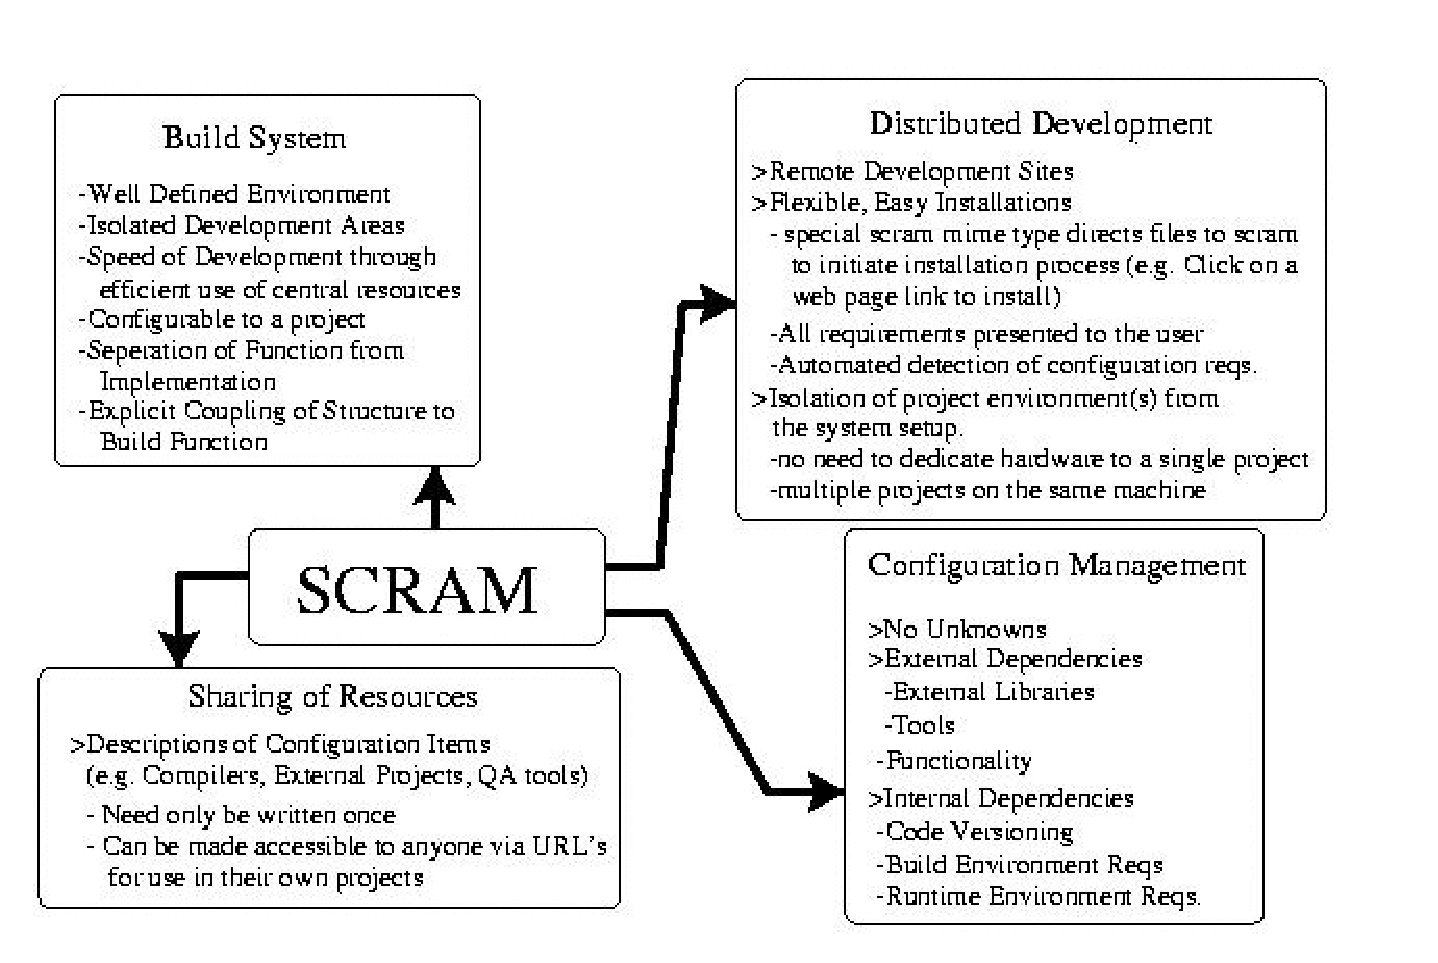
\epsfig{file=images/scram.eps, width=\linewidth}
      \caption[A SCRAM overview.] 
      {A SCRAM overview.}
      \label{f:SCRAM}
    \end{center}
  \end{figure}
\end{latexonly}

\ni In summary, \scram\ can provide
\begin{itemize}
\item project installation with a click on a web page;
\item control of the build environment, including dependency tracking;
\item fully configurable build operations, including default operations;
\item abstraction of logical build elements from the implementation details;
\item re-use of configuration management elements between projects.
\end{itemize}


\section{The Structure of This Guide}

This document can be broken down as follows: firstly,
Chapter~\ref{ch:install} gives some details on how to obtain \scram\
and instructions on how to create a local installation.
Chapter~\ref{ch:creatingprojects} contains all information necessary for
administrators (or users wanting to use \scram\ privately) to
create new projects using \scram\ as the management tool, and to
maintain them. The various types of project configuration files, and
the purposes of each (with use cases), are also described.
Chapter~\ref{ch:examples} serves as a resource for developers who
use \scram\ in their environment, providing some examples and tips covering topics
like changing tool configurations or adding new external tools in a
private area.

\ni Finally there is a summary page containing help for usage for all of
the currently supported \scram\ commands (p~\pageref{ch:quickhelpguide}).

\newpage % Start on a fresh page

%%% Local Variables:
%%% mode: latex
%%% TeX-master: "SCRAM-manual"
%%% End:

%%____________________________________________________________________ 
%% End of Introduction.tex
%%____________________________________________________________________ 
%%  

%%____________________________________________________________________ 
%% File: Installation.tex
%%____________________________________________________________________ 
%%  
%% Author: Shaun ASHBY <Shaun.Ashby@cern.ch>
%% Update: 2005-11-02 17:05:05+0100
%% Revision: $Id: Installation.tex,v 1.4.2.1 2007/03/02 13:54:00 sashby Exp $ 
%%
%% Copyright: 2005 (C) Shaun ASHBY
%%
%%--------------------------------------------------------------------
\chapter{Obtaining and Installing SCRAM}
\label{ch:install}\index{SCRAM!obtaining and installing}
The procedure for creating a central or local \scram\ release is
straightforward. Normally, these steps would be performed by computing
administrators but a user can also easily install \scram\ on his/her machine.
The installation uses the standard tool\texttt{configure}, which can be run to create a Makefile.

\section{Downloading and Installing from CVS}
\index{SCRAM!downloading}

Here is a guide to installing \scram. The sources can be installed
anywhere (read access is required of course); the final installed
\scram\ script must be locatable in the user path. The prerequisite
Perl toolkit for handling templates is automatically downloaded and
installed inside the source code tree so it is no longer necessary to
support options to specifiy where it is located. This is the
installation recipe:

\begin{enumerate}
\item Create a directory \texttt{SCRAM} in which you wish to keep your
  \scram\ installation,\mbox{}
  
  \eg \texttt{mkdir SCRAM}
  
\item Change to the installation directory created above,\mbox{}
  
  \eg \texttt{cd SCRAM}
  \index{CVSROOT}  
\item Set the environment variable \texttt{CVSROOT} to point to the
  CVS repository:\mbox{}

  \scramcvsrepository
  
  Use \texttt{export} or \texttt{setenv} depending on whether your
  shell is \texttt{zsh} or \texttt{tcsh}.
  
\item Log into the CVS server as user \textit{anonymous} (password is
  \texttt{98passwd}):\mbox{}
  
  \texttt{cvs login}
  
\item Check out the version of \scram\ (for example, \thisrelease)
  required:\mbox{}
  
  \texttt{cvs co -d \thisrelease~ -r \thisrelease ~SCRAM}
  
  Once a version of \scram\ has been installed, installation 
  of any other version is achieved easily using the command\mbox{}
  
  \texttt{scram version} \textit{new-version}
  
  The final step is to run \texttt{autoconf} and \texttt{configure}
  with the required options.
  
\item Go to the \texttt{Installation} directory of the version you have
  just checked out,\mbox{}
  
  \eg \texttt{cd \thisrelease/Installation}
  
\item Run \texttt{configure}, supplying any options required for your installation.\mbox{}
  
  Several templates for the main script (\texttt{scram.pl.in}), the
  install Makefile (\texttt{Makefile.in}) and for a local site package 
  (\texttt{SCRAM\_SITE.pm.in}) are processed.
  The site-dependent settings come from \texttt{SCRAM\_SITE.pm.in} and 
  their values are passed using options to \texttt{configure}. This
  template can be modified as desired to support features needed at each site.
  
  The \texttt{configure} script supports the following options:
  
  \begin{itemize}
  \item location of the Perl executable\mbox{}\\ 
    (\texttt{--with-perlexe=LOC}).
    
  \item directory where the SCRAM database file \texttt{project.lookup}
    is located\mbox{}\\ (\texttt{--with-scramdb-dir=DIR}).
    
  \item the name of the site, 
    \texttt{SCRAM\_SITENAME} (\texttt{--with-sitename=SITE}).
    
  \item the name of the installed SCRAM script in the installation directory\mbox{}\\ 
    (\texttt{--with-install-name=NAME}).
    
  \item the directory where the SCRAM script will be located\mbox{}\\
    (\texttt{--with-install-dir=DIR}).
    
  \end{itemize} 
  A list of options can be viewed using the command \texttt{configure --help}.
\end{enumerate}

\ni Then run \texttt{make}~\texttt{install}.
The installation process will have created a script called
\texttt{scram} (the default name) in the install directory (normally \texttt{bin}).

\ni If you wish to use \scram\ directly through web page links you will
now need to configure your browser to use \scram.

\section{Configuring Netscape to Use SCRAM}\label{sec:webbootstrap}
\index{bootstrapping!using Netscape}
\index{bootstrapping!using a web browser}
This section assumes that you are using Netscape Navigator but should
also apply to most web-browsers. Follow the checklist below--

\begin{enumerate}
\item From the \textit{Edit} menu, select
  \textit{Preferences}\mylongrightarrow
  \textit{Navigator}\mylongrightarrow\textit{Helper Applications}
  
\item Click on \textit{New} in the \textit{Helper Applications} window and
  complete the form. For the \texttt{MIMEType} entry, type\mbox{}
  
  \textit{application/scram\_bootstrap}
  
\item Click on the application box to select it and enter
  
  \texttt{xterm -e scram --noreturn project -d \textsc{dir} -b \%s}
  
  where \textsc{dir} is the directory where you would like all
  downloaded projects to reside (this directory must exist already).
  
\item Click the \texttt{OK} box to save it.
\end{enumerate}

\ni Now, whenever you click on a project bootstrap file your browser
will start an \texttt{xterm} in which \scram\ will run the project
installation procedure.

\section{Controlling SCRAM Versions}
\index{SCRAM!controlling versions of}
The version of \scram\ used can be easily changed by using \scram\
itself. The current version will be displayed by typing the command

\texttt{scram version}
 
\ni which will return a string with a format like \texttt{V1\_X\_X},
where the \texttt{X}'s are digits representing the major and minor
release numbers.  To switch to a different version, say \lastrelease, the
command would be\mbox{}

\texttt{scram version \lastrelease}.

\ni If the specified version already exists in the central
installation directory, it will be used. Otherwise, \scram\ will
attempt to download the requested version from the CVS repository.
The parameters for accessing a CVS server can be made site-specific by
modifying \texttt{SCRAM\_SITE.pm.in} prior to following the
installation procedure described in the previous section.

\ni Installing a specific version will make that version the default
(unless the link name is changed to something other than \scram\ or
a different installation directory is chosen).
In any case, this version can be overridden by
setting an environment variable \texttt{SCRAM\_HOME} to point to the
top-level directory of the required version:\mbox{}

\eg \texttt{export SCRAM\_HOME=/home/user/SCRAM/\lastrelease}

\ni will force \scram\ to use version \lastrelease\ throughout the current
session.

\ni \scram\ can be made to automatically select the correct version to
use for a given project area, overridding any other version selection
mechanism. To turn this feature on, simply create the file
\texttt{scram\_version} in your project development/release
\index{\texttt{scram\_version} file}
configuration directory. The file should contain the required \scram\
version tag. Any \scram\ command issued in that area is then directed
to the correct version if it is installed. If the required version is
not installed then a warning is issued and execution of the command
continues using the current (default) version.

\section{The SCRAM Database} 
\index{SCRAM!project database}
\index{\texttt{SCRAM\_USERLOOKUPDB} variable}
\index{installing and removing projects}
\index{\texttt{scramdb} directory}
\index{\texttt{project.lookup} file}
The \scram\ database file is called \texttt{project.lookup} and 
contains lookup tables for the various projects that may be 
installed on your system. The database is read
during a \texttt{scram list} command.  Usually, the database file
lives in the \texttt{scramdb} directory of
your \scram\ installation area and is accessible to all \scram\
versions. The database directory is created automatically at
installation time. The default location can be overridden with the
environment variable \texttt{SCRAM\_USERLOOKUPDB} which should be the
full path to the \texttt{project.lookup} file.

\begin{description}
\item[Installing a project in the database]\mbox{}\\
  A project can be installed into the database using the command

\begin{scramcmd}{install}
  \inbrackets{project\_name}~\inbrackets{project\_version}
\end{scramcmd}

\ni This command is usually executed in the project area of the
project (and version) to be installed.  If the project name and
version are given then these will be used in the database in place of
the project defaults.


\item[Removing an installed project from the database]\mbox{}\\
  A project can be removed from the database using the command

\begin{scramcmd}{remove}
  \inbrackets{project\_name}~\inbrackets{project\_version}
\end{scramcmd}

\ni This command can be executed anywhere but will only work if the
user has write permissions on the \texttt{project.lookup} file.

\index{linking other SCRAM databases}
\item[Linking other databases]\mbox{}\\
  Other databases can be linked to the local installation database
  using the command

\begin{scramcmd}{db link}
  ~\inbrackets{otherdb}
\end{scramcmd}

\ni This is often useful if a local copy of a project is maintained
for development but a released project is required for access to
configuration information and libraries. All projects listed in the
linked database will be shown by \texttt{scram list}.  Note that
\texttt{scram install} and \texttt{scram remove} commands will not
affect databases that are linked in.
\end{description}

\section{Supporting Multiple Architectures}

The site \scram\ installation can be customised to support multiple
architectures (where the architecture is dependent only on the
operating system specifics). Architectures that reflect a combination of
compiler, compiler version and \texttt{OS} will be supported in later
releases and are only supported as hard-coded strings.

\ni The architecture can be determined automatically and is not limited to
the mechanism used in \texttt{V0} versions of \scram\ which use only
\texttt{uname} and required the environment variable
\texttt{SCRAM\_ARCH} to be set to change to another architecture. 
A principal check uses \texttt{Perl} internal variables to
determine the name of the current platform. This value is then
compared to an architecture map found at the end of
\texttt{SCRAM\_SITE.pm.in} which can be freely edited-- \textit{before
running the install procedure above}-- to support any
desired architecture on which \texttt{Perl} will run. 
The architecture map data looks like this:
\begin{verbatim} 
__DATA__; # Signals end of package
######################################################
#                                                    #
# These are the architecture mappings for this site  #
#                                                    #
######################################################
linux:&linux_check(2,3,4,"intel") && &is_slc_version(4) && &is_64bit():"slc4_ia64_gcc345"
linux:&linux_check(2,3,4,"amd") && &is_slc_version(4) && &is_64bit():"slc4_amd64_gcc345"
linux:&linux_check(2,3,2,"amd") && &is_slc_version(3) && &is_64bit():"slc3_amd64_gcc345"
linux:&linux_check(2,3,4,"intel") && &is_slc_version(4):"slc4_ia32_gcc345"
linux:&linux_check(2,3,2,"intel"):"slc3_ia32_gcc323"
darwin:&check_is_osx_panther():"osx103_gcc33"
darwin:&check_is_osx_tiger() && &is_ppc() :"osx104_ppc_gcc40"
darwin:&check_is_osx_tiger():"osx104_ia32_gcc40"

\end{verbatim}

\ni The first element in each line of data is the native platform. The
second element is the name of a Perl subroutine (which can be
customised to suit), found in \texttt{SCRAM\_SITE.pm}, which will 
be run and will return true or false depending on whether some criteria (\eg versions of
\texttt{glibc}, the name of an \texttt{OS} release \etc) are satisfied. If they
are, the final element will be returned as the name of the
architecture. This will be set once as soon as \scram\ is run.
Setting the environment variable \texttt{SCRAM\_ARCH} or using
\texttt{scram -arch X <CMD>} will override this value.
Combinations of subroutines can be run also as in the second example above.
Any number of architectures can be listed but the last set
of parameters that fully match will be used to give the current
architecture name.

\newpage % A new page please

%%% Local Variables:
%%% mode: latex
%%% TeX-master: "SCRAM-manual"
%%% End:

%%____________________________________________________________________ 
%% End of Installation.tex
%%____________________________________________________________________ 
%%  

%%____________________________________________________________________ 
%% File: CreatingProjects.tex
%%____________________________________________________________________ 
%%  
%% Author: Shaun ASHBY <Shaun.Ashby@cern.ch>
%% Update: 2005-11-02 17:05:54+0100
%% Revision: $Id: CreatingProjects.tex,v 1.6.2.1 2007/03/02 13:54:00 sashby Exp $ 
%%
%% Copyright: 2005 (C) Shaun ASHBY
%%
%%--------------------------------------------------------------------
\chapter{Creating SCRAM-Managed Projects}\label{ch:creatingprojects}
\index{SCRAM!creating projects}
\index{creating SCRAM projects}

A \scram\ project is a releasable unit covering a particular software
domain, for example an analysis framework, event simulation or reconstruction.
Libraries and binary executables are the typical basic build products and these
can have separate storage areas. A configuration directory contains all the
files necessary to allow \scram\ to configure a dedicated project
release area for a version of the project. External requirements are
configured automatically. 
The structure of a project can be freely chosen since \scram\ does not
impose restrictions on project structure: it is
easy to modify \scram\ build behaviour according to site conventions.

\ni Generally, a project is subdivided into \texttt{subsystems} and
\texttt{packages} according to the tree structure of the source code
directory. Dependencies are expressed in terms of packages
where a package is typically built into a shared library: in fact,
the build products that correspond to a certain set of source files in
a certain location can be freely modified to suit the project. 
The principal reason for assuming (or enforcing in some cases) that
packages map to libraries is to enable proper dependency tracking and
automatic ordering of build operations. From Version 1.0 of \scram, 
this feature is fully supported both internally (to establish correct library
ordering in linker information) and via \texttt{gmake} which controls
the build ordering once the dependency information is correctly
obtained by \scram.

\ni Source files and header files have separate directories appearing under
\texttt{src} and \texttt{interface} or \texttt{include} respectively.
An additional directory called \texttt{test} can be used as a location 
to build binary executables for testing. Likewise, other directories 
can be used as locations to define other build products, for example 
\texttt{bin} or \texttt{app} for binary executables and applications 
which should be released as project deliverables.

\begin{figure}[htb]\index{project structure!recommended}
  \begin{center}
    \leavevmode 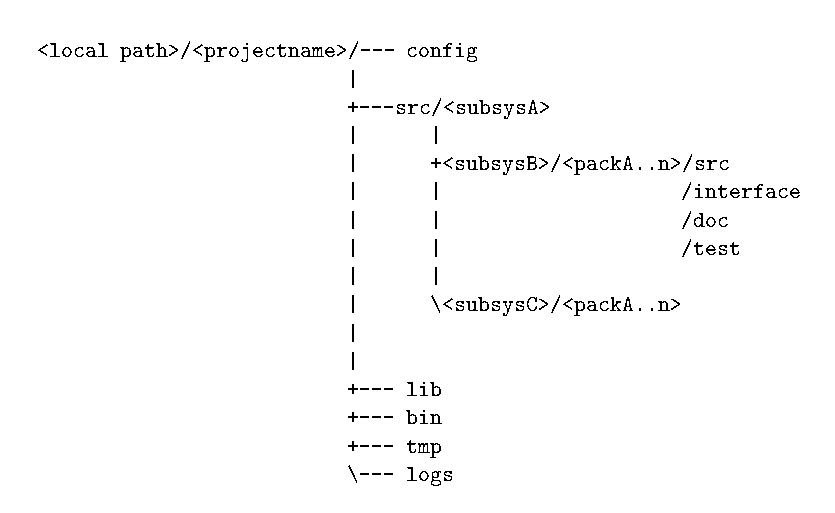
\epsfig{file=images/projectstructure.eps, width=\linewidth}
    \caption{Recommended \scram\ project structure. The directories
      \texttt{tmp} and \texttt{logs} are created
      automatically and directories for build products 
      like \texttt{lib} and \texttt{bin} 
      are created as appropriate given instructions 
      read from a project build file.}
    \label{fig:recprojstruct} 
  \end{center}
\end{figure}

\ni The corresponding \scram\ project structure consists of a directory
tree like that shown in Figure~\ref{fig:recprojstruct}.

\ni This chapter describes some of the important internal configuration aspects of
\scram\ that are used to define projects and should provide all the
information required for administrators and developers alike to
configure a \scram-managed project.

\section{SCRAM Project Components}

Every \scram\ project has documents to describe it and a code
repository from where these documents, and project source code, can be
accessed using a version management system.
The two elements are described in the following sections.

\subsection{Configuration Documents}\label{sec:scramconfigdocs}
\index{SCRAM!project configuration files}

\ni There are two types of project areas:
\begin{itemize}
\item \texttt{Releases} which are normally installed in a central location.
\item \texttt{Developer Areas} which are areas that are cloned from
  centrally installed releases but allow private access for software 
  development with the same controlled configuration as the release.
\end{itemize}

\ni The processes for initialising areas in each of these cases is different.
Each project must have a unique version, a name and a tool
configuration from which interfaces to external software can be
established. These interfaces express external dependencies in the
same way as individual packages in the project or release area of the
project. Their definitions are contained inside a toolbox and
list all settings needed by the \scram\ build or runtime environments (for
example, \texttt{INCLUDE} paths, libraries provided by the tools or \texttt{PATH} elements
which should be added to the user environment).

\ni Configuration instructions for \scram\ are passed using documents called
\texttt{ActiveDocs} which are \texttt{XML} files (the support for
\texttt{XML} document parsing is a new feature in this release).
These are web-enabled mark-up documents, each being associated with a
download and cacheing mechanism that is accessed using a \texttt{URL}. This
\texttt{URL} can behave like a normal \texttt{WWW} \texttt{URL} or can be a file or a
path to a \texttt{CVS} server. A number of \texttt{ActiveDoc} markup tags are
defined, some of which are common to all types of document; some tags
are specific for their application and only used in a particular class
of document.  An \texttt{ActiveDoc} document must begin with a special
statement that informs \scram\ what sort of document it is and how it
should be parsed; each type of statement is specific to a class of
functionality. The parent tag
\begin{tagprint}
  \lbkt\texttt{doc} type=\textit{"type"} version=\textit{"version"}\rbkt
\end{tagprint}
\ni is always the first line of the document after the \texttt{XML}
document header
\begin{tagprint}
  \xmldocheader
\end{tagprint}

\ni The \texttt{doc} type is set according to the \scram\ parsing
class and all \scram\ \texttt{XML} documents must end with a corresponding
\lbkt$/$\texttt{doc}\rbkt tag.

\ni There are three main different classes of \texttt{ActiveDoc} document
that are needed to configure a project: \texttt{BootStrapProject},
\texttt{RequirementsDoc} and \texttt{ToolDoc}. These classes are
described next.

\subsubsection{The BootStrapProject Class}\label{sec:bootstrapclass}
\index{\texttt{BootStrapProject} class}
A single document describes how the project should be structured and
which tools should be configured. Usually referred to as a \texttt{bootstrap} file, it must start with
the statement\index{project \texttt{BootStrapFile}} 
\index{bootstrap file}
\begin{tagprint}
  \lbkt\texttt{doc} type=\texttt{"Configuration::BootStrapProject"}
  version=\textit{"1.0"}\rbkt
\end{tagprint}
\ni The name of this file is completely arbitrary. The function of
the bootstrap document is to define the name and version of a project
and to tell \scram\ from where it can download the configuration and
source code files, and where to put them inside the project release
area. There must be a bootstrap file in every \scram\ project.

\ni The markup tags specify a path to a \texttt{CVS} server, the name of the
project requirements document and the location of the project
configuration directory within the project area.  The available markup
tags are as follows--
\index{\texttt{BootStrapProject} markup tags}
\index{\texttt{BootStrapFile} markup tags} 
\begin{description}
\item[\lbkt\texttt{project} name=\textit{"name"} version=\textit{"version"}\rbkt~\tagend{project}]\mbox{}\\
  Specify the name an version of the project. The version should be a
  valid \texttt{CVS} symbolic tag which must exist on all files in the
  configuration directory and the project source code. Explanatory
  text can be put between the \lbkt\texttt{project}\dots\rbkt tags: this
  text will be printed to the screen when bootstrapping the project.
\item[\lbkt\texttt{config} dir=\textit{"dirname"}$/$\rbkt]\mbox{}\\
  Specify the name of a directory relative to the top of the project
  area where the configuration files can be found.
\item[\lbkt\texttt{base} url=\textit{"baseurl"}\rbkt~\tagend{base}]\mbox{}\\
  A common element in multiple \texttt{URL}s, such as a \texttt{CVS} server name, is
  supplied using the base tag. The \texttt{URL} type can be \texttt{cvs:}
  (using a \texttt{CVS} repository) or \texttt{file:} (a standalone file). Any
  \texttt{URL} specified between the start and end base tags will be merged
  with the \texttt{URL} \textit{baseurl} according to the following merge
  rules:
  \begin{itemize}
  \item A merge will only take place if the \texttt{URL} and \textit{baseurl}
    types match, \eg both have type \texttt{cvs:} or \texttt{file:}
  \item The base server name is taken if it isn't already defined
  \item The \textit{baseurl} path is prepended to any \texttt{URL} specified
  \item Variables provided in the base parameter list are only added
    if not already defined, \eg definition of the directory name when
    downloading the configuration files
  \end{itemize}
\item[\lbkt\texttt{download} url=\textit{"url"} name=\textit{"dirname"}$/$\rbkt]\mbox{}\\
  Each \texttt{URL} will be merged with the base \texttt{URL} defined in a
  \tagstart{base} tag and treated as a download location which is
  passed to \texttt{CVS} for checking out files from a repository. The name of
  the destination directory will be \textit{dirname}, and will be
  located relative to the top of the project area.
\item[\lbkt\texttt{requirementsdoc} name=\textit{"docname"}$/$\rbkt]\mbox{}\\
  Specify the name of the project requirements document. The path is
  relative to the top of the project area.
\end{description}

\subsubsection{The RequirementsDoc Class}\label{sec:requirementsdocclass}
\index{\texttt{RequirementsDoc} class}

To make external products available in a project area and be able to
link against external libraries, a requirements file is used. This
file starts with the statement\index{requirements file}
\begin{tagprint}
  \lbkt\texttt{doc} type=\texttt{"BuildSystem::Requirements"}
  version=\textit{"2.0"}\rbkt
\end{tagprint}
\ni and specifies the external tools and their corresponding versions
that should be configured. The requirements file provides information
for \scram\ to use when downloading the tool descriptions from the
toolbox \texttt{CVS} repository. If more than one version of a tool is defined,
the first one is taken as the default.
The following tags are available:

\begin{description}     
\item[\lbkt\texttt{require} name=\textit{"name"} version=\textit{"version"} url=\textit{"url"}$/$\rbkt]\mbox{}\\
  Specify the name and version of a required tool. The \texttt{URL} should
  point to a \texttt{ToolDoc} that describes the tool. Base \texttt{URL} tags
  (\lbkt\texttt{base}\rbkt\ldots) can be used to modify the \texttt{URL}.
\item[\lbkt\texttt{include} url=\textit{"url"}$/$\rbkt]\mbox{}\\
  This is for \texttt{URL} document preprocessing.\texttt{ActiveDocs} provide
  an equivalent of the \texttt{C}-preprocessor
  \texttt{\#include}
  \index{\texttt{include} directive}
  directive that is web-aware. In this way, it is possible to assemble
  a document from many components that are maintained at different
  locations.  A common configuration file containing multiple tool
  \lbkt\texttt{require}\rbkt statements can be included in this way.
\item[\lbkt\texttt{architecture} name=\textit{"arch"}\rbkt~\tagend{architecture}]\mbox{}\\
\index{architecture tags}
\index{SCRAM!architecture}
\index{\texttt{SCRAM\_ARCH}}
  \ni The \textit{arch} is an architecture tag which limits certain
  functionality only to a specific operating system. This
  architecture is determined automatically by \scram. Unlike previous
  versions, the mechanism to determine the architecture name is
  defined in \texttt{Installation/SCRAM\_SITE.pm} and is fully
  customisable. Internally, \scram\ sets a variable called \texttt{SCRAM\_ARCH} to
  whatever is determined as the architecture string. This string can
  then be used as \textit{arch} (either the full architecture name or an
  abbreviation will match).

\item[\lbkt\texttt{download} url=\textit{"url"}$/$\rbkt]\mbox{}\\
  Specify a link to download information for the tool.
\item[\lbkt\texttt{select} name=\textit{"name"}$/$\rbkt]\mbox{}\\
  Select a tool from a list of available tools.
\end{description}

\subsubsection{The ToolDoc Class}\label{sec:tooldocclass}
\index{\texttt{ToolDoc}!class}
An external tool is described using a tool description file called a
\texttt{ToolDoc}. When a tool is required, a certain version of that
tool is configured by \scram\ in the project area.  A tool description
begins with the statement\index{\texttt{ToolDoc}}
\begin{tagprint}
  \lbkt\texttt{doc} type=\texttt{"BuildSystem::ToolDoc"} version=\textit{"1.0"}\rbkt
\end{tagprint}
\ni The \texttt{ToolDoc} describes such things as the default location
of the tool on the system, the names of libraries to be used when
linking against the tool and environment variables that must be set at
runtime. The external dependencies of the tool are also declared.

\ni The following tags are available in \texttt{ToolDoc}s:
\index{\texttt{ToolDoc}!valid markup tags}
\begin{description}     
\item[\lbkt\texttt{tool} name=\textit{"name"} version=\textit{"version"}\rbkt\tagend{tool}]\mbox{}\\
  Specify the name and the version of the tool that is being
  described. Everything between these tags relates to version
  \textit{version} of the tool.
\item[\mbox{\lbkt\texttt{environment} name=\textit{"variable"}
    {[}default=`\textit{"def"}' \textbf{or} value=`\textit{"value"}'{]}
    type=\textit{"type"}$/$\rbkt}]
  Set up a variable in the \scram\ environment for this tool.
  Either `value' or `default' can be set
  to provide the appropriate path for the variable but not both.
\item[\mbox{\lbkt\texttt{runtime} name=\textit{"variable"}
    {[}type=`\textit{"path"}'{]}
    {[}handler=`\textit{"warn","error"}'{]} $/$\rbkt}]\mbox{}\\
  Define a runtime variable which should be set in the users' shell
  environment. The optional variable type \textit{type} can be set
  to \texttt{path} for a path-like variable, \eg
  \texttt{\$PATH} or \texttt{\$LD\_LIBRARY\_PATH}, at runtime.
  If the handler option \textit{handler} is set to \texttt{warn},
  \scram\ will not pause and prompt for a value for the runtime
  variable if the value is incorrect (for example, if the path is
  missing because the directory has not yet been created).
\item[\lbkt\texttt{use} name=\textit{"tool name"}$/$\rbkt]\mbox{}\\
  Specify that the tool has a dependency on another external tool.
\item[\lbkt\texttt{lib} name=\textit{"libname"}$/$\rbkt]\mbox{}\\
  Specify the name of a library belonging to the tool. Note that the
  preceding `lib' or extension are not required.
\item[\tagstart{client}~\tagend{client}]\mbox{}\\
  Any \inbrackets{environment} definition between these tags will be
  checked as a directory location on the client machine.
  The presence of all libraries defined by \lbkt\texttt{lib}\rbkt tags 
  will be checked for automatically. The \texttt{client} tags should
  only contain \texttt{environment} tags: if an environment is
  architecture-specific, the \texttt{client} block must be included in
  the architecture block and not the other way around.
\item[\tagstart{makefile}~\tagend{makefile}]\mbox{}\\
  These tags delimit \texttt{gmake} makefile content intended for
  inclusion in the build system associated with the tool. It is preferable to use
  text templates (or modify existing templates) if the content to be
  added is more than a single line (\eg a variable definition).
\item[\lbkt\texttt{flags} \texttt{NAME}="definition"\rbkt]\mbox{}\\
  Extra compiler flags can be specified which will be added to the
  global compiler flags if the tool defining them is required
  globally, or added to the compiler flags for a package if the tool
  is required there.
\end{description}

\ni Note that all environment variables can be referred to by others in
addition to internal \scram\ variables like \texttt{\$SCRAM\_ARCH}, the
tool name \texttt{\$SCRAMtoolname} and the version
\texttt{\$SCRAMtoolversion}.

\subsection{The CVS Infrastructure}\label{sec:configuringCVSinf}
\index{CVS repositories}
\index{CVS repositories!setting up for a new project}
All code management within \scram\ uses \texttt{CVS}, a versioning system 
derived from \texttt{RCS}.\footnote{However, \scram\ does
not fully depend on CVS: another tool could be used instead if
required at a later date.}
Every project consists of source code and \scram\ project
configuration files which are imported into a \texttt{CVS} repository which
has a directory structure mirroring the structure of the project itself.
\begin{figure}[ht]\index{CVS repositories!recommended structure}\index{CVSROOT}
  \begin{center}
    \leavevmode 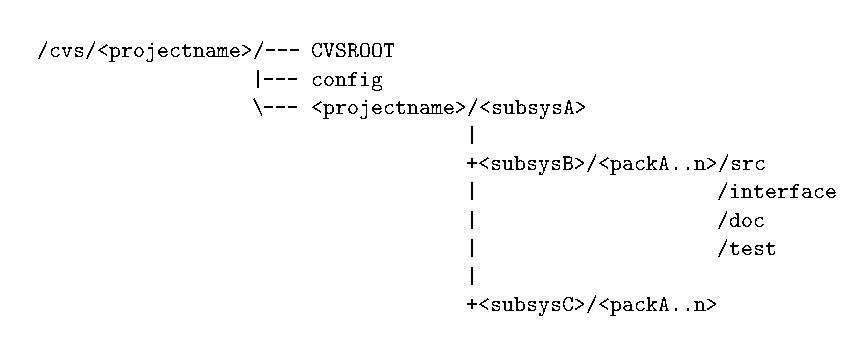
\epsfig{file=images/projectCVSstructure.eps, width=\linewidth}
    \caption{Recommended CVS repository structure for a \scram\
      project. The directory \texttt{CVSROOT} contains CVS information
      and is created automatically when initialising the CVS repository.}
    \label{fig:recprojstructCVS}
  \end{center}
\end{figure}
The typical repository structure, based on the project structure
described earlier, is illustrated in Figure~\ref{fig:recprojstructCVS}.
%
\subsubsection{CVS Authentication}\label{sec:CVSauth}
\index{CVSROOT!authentication settings and}
\index{CVS authentication options}
To access the CVS repository, an authentication method must be chosen
and specified in the \texttt{CVSROOT} environment variable. There are
currently two supported methods for file checkout in \scram:
\texttt{pserver:}, standard anonymous checkout, and \texttt{local:},
using a CVS repository on a local filesystem on the current machine
rather than a dedicated server accessible only via a network
connection. 

\subsubsection{Importing the Code for New Projects}\label{sec:importingcode}
\index{CVS repositories!importing files to}
\ni Moving source code into a repository when creating a new project
is explained in detail in the CVS manual but a brief description is
given here. Once project source code exists in a suitable directory tree, the
whole project can be imported into a CVS repository using 
the \texttt{cvs import} command. Initially, the \texttt{CVSROOT}
environment variable must be set and
the repository created using the command \texttt{cvs init}.
To make life easier when defining download paths in bootstrap
files, the \texttt{CVSROOT} for project \texttt{MyProject} on a local
filesystem would look like

\begin{list}{}
\item\texttt{/local/path/cvs\_repository/MyProject} 
\end{list}

\ni and would be set before importing the code. Import the
configuration directory (and contents) first

\begin{indentprint}\texttt{cd config}\end{indentprint}
\vspace{-3mm}
\begin{indentprint}
  \texttt{cvs import -m "First import of my project config" config V1-0 V1-0}
\end{indentprint}

\ni and then repeat this step for the project sources:

\begin{indentprint}\texttt{cd MyProject}\end{indentprint}
\vspace{-3mm}
\begin{indentprint}
  \texttt{cvs import -m "First import of my project src" MyProject V1-0 V1-0}
\end{indentprint}

\ni Once this has been done and assuming that the import was
successful, the original sources can be removed and then restored from \texttt{CVS}
using \texttt{cvs co MyProject}.

\subsection{The SCRAM Toolbox}\label{sec:toolboxrep}
\index{SCRAM!toolbox CVS repository}
\index{CVS repositories!for tool descriptions}
A separate \texttt{CVS} repository must exist which contains 
documents describing external tools: these are components of a {\em toolbox}. 
This is referred to as the \scram\ toolbox.
Each tool has a \texttt{ToolDoc} in which every
version of the tool that can be used in a project environment is
described. Any environment or makefile variable needed to use the
external software is declared in the file and interpreted by \scram\ as
a variable to be set up when creating the project area for the first
time, or installing a new version of the tool into an existing area.
A global configuration file (called
`the configuration') indicates which tools and the corresponding versions that can
be downloaded by \scram\ and used in project-space. The toolbox is
tagged with a \texttt{CVS} symbolic tag which is used to \textit{freeze} the
configuration: this tag is then specified in the project
\texttt{RequirementsDoc} as the version to download.
There is no requirement for a particular structure for the toolbox 
but including at least the following is recommended:

\begin{description}
\item[\textbf{Compiler Tools}]\mbox{}\\
  Any number of programming languages can be supported (for example \texttt{C},
  \texttt{C++}, \texttt{Java} or \texttt{Fortran}). The top-level
  \texttt{BuildFile} for the project should select the compilers that should
  be configured globally (compilers can also be selected for use only at
  the package level where they are required).
\item[\textbf{External Software}]\mbox{}\\
  Each external software package to be used by a project should have a
  unique tool description file which defines the required version of
  the tool.
\item[\textbf{Project Software Releases}]\mbox{}\\
  Tool descriptions for all projects that provide libraries to be used
  by other projects or tools should be created.
\item[\textbf{A Configuration File}]\mbox{}\\
  The most important element in the toolbox. The 
  configuration describes the available tools and 
  versions of these tools that are to be used in a
  project area.
\end{description}

\section{Creating a Project Release Area}\label{sec:creatProjArea}
\index{Project areas!creating new}

The starting point in a software development cycle is to create a project
release to estabish a baseline for further development. 
A \scram\ project must have, at least, the following configuration
files in a configuration directory to properly define the project:
\begin{description}
\item[\texttt{boot.xml}]\mbox{}\\
  For bootstrapping the project. This will relate a specific project
  version with the relevant source code version and define a
  requirements file to be read to select external products.
\item[\texttt{requirements.xml}]\mbox{}\\
  The requirements file containing information to be passed to the
  configuration manager for setting up external tools. A \texttt{CVS}
  symbolic tag for a released configuration specifies which tools and
  version should be downloaded from the toolbox repository.
\item[\texttt{config/BuildFile.xml}]\mbox{}\\
  The top-level \texttt{BuildFile}, containing project-wide default settings for
  export of external tools, build product storage and global compiler settings. 
\end{description}

\ni These files are normally kept in a directory called
\index{\texttt{config} directory}
\index{project configuration directory}
\texttt{config} (the name of the directory can be changed using a
directive in the boot file).  A \scram\ command exists
which can be used to grab basic template files for a new project.
Typing

\begin{scramcmd}{project -template}\end{scramcmd}

\ni will download some basic project configuration files to a
directory called \texttt{config} in the current directory. These
should be edited to suit and imported into the project CVS repository
(see Section~\ref{sec:configuringCVSinf}). Once these configuration
files exist, they must be tagged with a \texttt{CVS} symbolic tag that matches the name
and version of the project (for example \texttt{myProject\_1\_0}).
All project source code must have the same global \texttt{CVS} tag (this is
especially important if you want the bootstrap mechanism to also
download source code).

\ni Creating the project area is very easy- just type the command

\begin{scramcmd}{project -b config/boot.xml}\end{scramcmd}

\ni indicating the location of the bootstrap file after the \texttt{-b} 
option, and that's it. \scram\ will set up the tools automatically
using the settings in the default lookup file \texttt{tools-X.conf}
found in \texttt{config/site}, or whichever lookup file is
specified on the command line.

\ni Two subdirectories are created in the project area as part of the
initialisation: \texttt{config} and \texttt{.SCRAM}. All files used
for bootstrapping and the build system are contained in
\texttt{config}, downloaded directly from the \texttt{CVS} repository. The
important project information is contained in the \texttt{.SCRAM}
subdirectory
\label{sec:dotSCRAMcontents}
\index{\texttt{.SCRAM} directory} so this must not be renamed or
deleted. A closer look at the contents of the \texttt{.SCRAM}
directory reveals the following subdirectories and files:

\small{
\begin{verbatim}
 ObjectDB/
 Environment
 cache/
 InstalledTools/
 slc3_ia32_gcc323/
 DirCache.db
\end{verbatim}
}\normalsize

\ni The directories \texttt{ObjectDB}, \texttt{cache} and
\texttt{InstalledTools} store tool description files as they are downloaded
from the \texttt{CVS} repository prior to being parsed by the setup mechanism.
Once each tool has been configured for use in the current environment,
the tool information is stored in the tool cache in
a directory for the architecture (in this example,
the architecture is \texttt{slc3\_ia32\_gcc323}). The file
\texttt{Environment} contains information required about the project
by \scram. The file content for a typical project \texttt{TEST} version 
\texttt{TEST\_1\_0} looks like this: 

\small{
\begin{verbatim}
SCRAM_PROJECTNAME=TESTING
SCRAM_PROJECTVERSION=1.0
SCRAM_TOOLBOXVERSION=CMS_145a_2
SCRAM_PROJECT_TIMESTAMP=Wed-28-Feb-2007 14:10:22
LOCALTOP=/home/t/work/projects/TESTING_1.0
\end{verbatim}}\normalsize 
%
\ni These entries are also defined as environment variables, visible in
the runtime and build environments. There will also be content like
\index{\texttt{RELEASETOP} settings}
\small{
\begin{verbatim}
RELEASETOP=/home/t/work/releases/TESTING_1.0
SCRAM_PROJECT_RELEASE_TIMESTAMP=Tues-27-Feb-2007 16:12:28
\end{verbatim}
}\normalsize

\ni in a developer area, informing \scram\ that the central area containing libraries and
header files should be used first, before any of the contents of the
current area. The timestamp of the release is also shown.

\ni The file \texttt{DirCache.db} is the timestamp cache file and
contains timestamp information for each file and directory in the
project source tree and configuration directory (\texttt{config}).
This will only exist when a build has run for the project.

\subsection{The Project Boot Process}
The principle of both the bootstrapping and tool setup is the same as
with previous versions of \scram. However, in the current version there is a fundamental
difference in the way that the tool data, before and after being set
up, is stored in the project.
All tool data is now cached in a file called \texttt{ToolCache.db} which is
stored in an architecture-dependent location inside the 
project (\ie under \texttt{.SCRAM/\$SCRAM\_ARCH}).

\begin{description}
\item[Tool downloading:]\mbox{}\\ 
  After tools have been downloaded to the local \scram\ cache (usually
  \texttt{.SCRAM/cache}), those tools selected in the \texttt{RequirementsDoc} will be
  set up. For each tool, a file \texttt{.SCRAM/InstalledTools/}\textit{toolname} will
  be created. At the same time, the contents of this file will be
  parsed and stored in the tool cache file. The order in which the
  \lbkt\texttt{select}\rbkt statements appear in the \texttt{RequirementsDoc} will be the order
  in which the tools are set up \textit{and} the order in which they appear in
  any path-like runtime variables. This is completely independent of the
  order in which tool files are downloaded (that is, the order in
  which the \lbkt\texttt{require}\rbkt statements appear in the tool
  configuration file, \ie \texttt{CMSconfiguration}).
  
\item[Tool Storage:]\mbox{}\\ 
  The cache file \texttt{ToolCache.db} replaces the numerous \texttt{*.dat} files that were previously
  located in the architecture-dependent directories under \texttt{.SCRAM}. 

\item[Tool Parse:]\mbox{}\\ Once the tool is parsed and set up (using input from
  \texttt{tools-CERN.conf}), a \texttt{ToolData} object holds the
  data within the cache. The tool object provides the methods to access the
  tool metadata.

%% Skip this part for now, since it's not particularly reliable!
%%
% \item[Other Project Setup:]\mbox{}\\
%   Setting up a project area which depends on another SCRAM-managed
%   project is now quicker and less prone to error since the entire tool
%   setup is copied to the new area. Only additional tools are set up in
%   the traditional way. Note that the SCRAM projects used in the
%   current project configuration must be installed in the scram database.
%%
\end{description}

\subsection{Standalone Project Areas}

Project areas can also be bootstrapped without having access to a
\texttt{CVS} repository or a version control system by using only local copies of the project
configuration files (and toolbox files, if required). This is ideal for fast prototyping.
There are two possible methods:

\begin{description}
\item[Method 1:]\mbox{}\\ 
Use a standalone configuration directory which be copied directly to
the new project area, with \texttt{CVS} used only in the requirements
file to specify where the tool configuration and tools should be
downloaded from.
In this context, "standalone" means that the download \texttt{URL} is
of type \texttt{file:}, rather than \texttt{cvs:}.
The requirements file does specify \texttt{cvs:} with the path to the
toolbox repository.

\item[Method 2:]\mbox{}\\ 
Use a standalone configuration directory and toolbox. Both the config
and the toolbox are normal directories on a local filesystem and only
the \texttt{file:} type of \texttt{URL} is used.
\end{description}

\ni Examples of the content of boot files, requirements files and a
standalone toolbox are given in Chapter~\ref{ch:examples}.

\section{Creating a Developer Area}\label{sec:SCRAMdevareas}
\index{using SCRAM developer areas}
\index{SCRAM developer area}

\ni A developer area is an isolated area where a developer can work on a
given project without affecting other developers. This area is
associated with a particular version of a project available centrally
from which it can use resources (\eg \texttt{\#include} files, libraries or
environment files and settings). Software developers can check out source code 
from \texttt{CVS} and \scram\ will build the products defined locally
and use these in place of those available in the
central release. All other products are transparently taken from the central project
release.

\ni To develop on a given project a copy of the project must be installed
at the developer site. Available projects can be viewed using the
command \texttt{scram list}. To create the developer space, the command

\begin{scramcmd}{project}
  \inbrackets{project\_name}~\inbrackets{project\_version}
\end{scramcmd}

\ni should be issued. The project name and version above are taken
from the list of \scram\ projects. The development area has the
structure and the same build environment as the base project.
Alternatively, a developer can bootstrap a project by first
checking out the \texttt{config} directory that matches the version of
the project that the developer are is to be based on and following the
steps described in Section~\ref{sec:creatProjArea}.
This can be implemented via a web interface such that a
source code distribution of the project can be obtained via a \scram\
download mechanism which can be enabled using any web browser. Follow
the instructions in Section~\ref{sec:webbootstrap} on page 
p\pageref{sec:webbootstrap} to do this. Once
correctly configured, a project can be installed using a single-click
operation in a browser window. 

\subsection{Using the Developer Area}\label{sec:usingscramdevarea}
\index{SCRAM developer area!using a}

Once the area has been created, the \texttt{src} directory can be
populated with the source code of interest. This step
involves \texttt{CVS} alone; usually, a module corresponds to a package and so
the whole module would be checked out from the \texttt{CVS} repository. This
would be achieved using the command

\texttt{cd src;}~\texttt{cvs co}~\textit{module}

\ni Note that the above command will check out the development
\texttt{HEAD}. To check out a fixed tagged version or the head of
another development branch, specify a \texttt{CVS} revision using the {\bf -r}
option:

\texttt{cd src;}~\texttt{cvs co -r}~\textit{version}~\textit{module}

\ni Once the sources are checked out, they can be edited as required
and committed to \texttt{CVS}.


\subsection{Obtaining Help}\label{sec:gettinghelp}
\index{getting help}
\index{\texttt{scram help}}
\index{\texttt{scram help} for specific commands}
Help can be obtained directly using the \scram\ global \texttt{help}
command, or by using the \texttt{help} option of a specific command.
For example,

\begin{description}     
\item[\texttt{scram help} or \texttt{scram -help}]\mbox{}\\
  will list all available \scram\ commands
\item[\texttt{scram} \textit{command} \texttt{-help}]\mbox{}\\
  will print the help for a specific command
\item[\texttt{scram build -help}]\mbox{}\\
  will print the help available for the current build location.
  Normally, this will show the available types of build that can be
  performed in the current directory.
\end{description}

\ni The short versions of the help command can also be used (\ie
\texttt{-h} instead of \texttt{--help}). 

\ni A summary of the \scram\ commands is available in Chapter~\ref{ch:quickhelpguide}.


\section{The SCRAM Runtime Environment}\label{sec:scramruntimeenv}
\index{SCRAM!runtime environment}
\index{runtime environment}
Each development area has an environment associated with it which is
related to the tools used at build-time (the \textit{configuration
  environment}) or project-wide defaults used at runtime (the
\textit{application environment}).  \scram\ establishes the build-time
environment through the parsing of the \texttt{ToolDocs} of the tools
in the configuration environment. The values of any variables that
describe paths to header files or required libraries are passed
automatically to the build system at build-time. Project-wide defaults
can be specified using a document called \texttt{Self.xml}, which is
located in project configuration directory and contains default
settings for variables that should be available globally in the
project area.
\index{SCRAM!runtime environment!viewing and setting}
\ni The current environment can be viewed using the command

\begin{scramcmd}{runtime}
  \marg{-sh}~(\textit{or}~\marg{-csh} for \texttt{tcsh} users)
\end{scramcmd}

\ni choosing the appropriate shell type flag according to the type of
shell in use. The runtime environment is not set automatically. To set
it, evaluate the command above using the shell \texttt{eval} function:

\begin{tagprint}
  \texttt{eval} `\texttt{scram runtime}~\texttt{-sh}` (\textit{or} \texttt{-csh})
\end{tagprint}

\ni This must be set manually when running an executable since it
sets the \texttt{LD\_LIBRARY\_PATH} and other environment
variables, as defined in the configuration documents of the
project.  All variables that are set also have an associated
\texttt{SCRAMRT\_xxxx} variable. This allows \scram\ to undo any
changes to the environment and facilitates the switching between
project areas without interference. The consistency checking is done
automatically.

\subsection{Constructing Runtime Environment Documents}\label{sec:constructingruntimedocs}
\index{SCRAM!runtime environment!constructing}
\index{constructing a runtime environment document}
A runtime document can be created for any application with the purpose
of defining any environment variables that might be required to run
the application properly. These might be special switches that control
how an application runs or settings of internal debugging or verbosity
levels. A variable can be defined in a runtime document using the tag

\begin{tagprint}
\lbkt\texttt{runtime} name=\textit{"variable"} value=\textit{"value"}
{[}type=\textit{"type"}{]} {[}handler=\textit{"warn","error"}{]}$/$\rbkt\mbox{}\\
\end{tagprint}

% \ni A good practise is to include some usage information between the
% \lbkt\texttt{runtime}\rbkt tags in the definition of the variable.
\ni All variables defined in a runtime document \texttt{filename} can be viewed using the command

\begin{scramcmd}{runtime}
  \marg{-sh}~(\textit{or}~\marg{-csh})~\marg{-f filename}
\end{scramcmd}

\ni or for a specific variable only using

\begin{scramcmd}{runtime}
 \marg{-sh}~(\textit{or}~\marg{-csh})~\marg{-f filename}~\marg{-info varname}
\end{scramcmd}

\ni The file \texttt{filename} is assumed to be located in the current directory.

\section{Interacting with the Configuration Environment}\label{sec:configurationtools}
\index{configuration tools}
Although all required external tools are automatically set up by the
\scram\ configuration manager in every project area, a developer may
want to change settings to suit a local system like a laptop computer.
\scram\ provides several commands to allow developers to easily view
the configuration environment and also to change it. The list of
configured tools available can be obtained using the command

\begin{scramcmd}{tool}
  \texttt{list}
\end{scramcmd}

\ni This will present a list like the one shown below: \footnotesize{
\begin{verbatim}
Tool list for location /home/t/work/projects/TESTING_1.0
++++++++++++++++++++++++++++++++++++++++++++++++++++++++

 cxxcompiler          3.2.3     
 f77compiler          3.2.3     
 ccompiler            3.2.3     
 clhep                1.9.2.3   
 aida                 3.2.1

\end{verbatim}
}\normalsize

\ni The settings for a tool can be viewed using the command

\begin{scramcmd}{tool}
  \texttt{info} \texttt{tool\_name}
\end{scramcmd}

\ni For example, the settings of the tool \texttt{zlib} would look like
this: \small{
\begin{verbatim}
Tool info as configured in location /home/t/work/projects/TESTING_1.0
+++++++++++++++++++++++++++++++++++++++++++++++++++++++++++++++++++++

Name : zlib
Version : 1.1.4
++++++++++++++++++++
SCRAM_PROJECT=no
ZLIB_BASE=/opt/lcg/external/zlib/1.1.4/slc3_ia32_gcc323
LIB=z
LIBDIR=/opt/lcg/external/zlib/1.1.4/slc3_ia32_gcc323/lib
INCLUDE=/opt/lcg/external/zlib/1.1.4/slc3_ia32_gcc323/include
LD_LIBRARY_PATH=/opt/lcg/external/zlib/1.1.4/slc3_ia32_gcc323/lib
\end{verbatim}
}\normalsize

\ni Another useful command can be used to extract the settings of
individual variables for a tool:

\begin{scramcmd}{tool}
  \texttt{tag} \texttt{tool\_name} \option{tag\_name}
\end{scramcmd}

\ni where \textit{tag\_name} is the name of a variable relevant for
the tool \textit{tool\_name}. If no tag name is given then all
variable names will be printed. If this command is used in the
following way

\begin{scramcmd}{tool}
  \texttt{tag} \texttt{zlib} \marg{INCLUDE}
\end{scramcmd}

\ni then \texttt{/opt/lcg/external/zlib/1.1.4/slc3\_ia32\_gcc323/include} will be printed.  This
is especially useful within shell scripts and avoids the need for
parsing the command output with shell utilities like \texttt{sed} or
\texttt{awk}.

\subsection{Changing Settings of Tools}\label{sec:changingtoolsettings}
\index{changing settings of tools}

The default settings of the installation can be changed at any time.
There are two modes available for setting up the tools: automatic and
interactive. The automatic mode is the default and will be used to set
up tools after a \texttt{scram project} command using a bootstrap file
has been issued. In this automatic mode, the \scram\ configuration
manager attempts to determine the correct values of the tool variables
using default locations, environment variables or checking other
already installed projects. Failing this, the user will be prompted to
enter a value using interactive mode.  Once a value has been chosen
for a path it will be checked to make sure that it exists. If it does
not, the user will be prompted to try again.

\ni Many of the common external tools used at CERN are installed in 
single locations. The automated setup mechanism can use a variable to
define a search path. This is the purpose of the tool lookup file (usually a file
called \texttt{tools-SITENAME.conf} where sitename is site-specific
and can be set when \scram\ is installed \footnote{Some examples of
  site names area CERN, LAPTOP, STANDALONE etc.}).  

The variable called \texttt{SCRAM\_BASEPATH} can be set to
point to the base directory of an external installation area as in the example
below. Variable expansion occurs automatically so this variable can be
used anywhere in a tool lookup file.
A lookup file for a system with \texttt{SCRAM\_ARCH} set to
\texttt{slc3\_ia32\_gcc323} starts with the following entries:

\small{
\begin{verbatim}
ARCHITECTURE:slc3_ia32_gcc323
SCRAM_BASEPATH:/opt/cms/external
\end{verbatim}
}\normalsize

An entry for a tool then looks like this:

\small{
\begin{verbatim}
TOOL:cxxcompiler:
   +CXX:/usr/bin/c++
   +CC:/usr/bin/gcc
TOOL:clhep:
   +CLHEP_BASE:$SCRAM_BASEPATH/clhep/1.9.2.3/slc3_ia32_gcc323
\end{verbatim}
}\normalsize

\ni When \scram\ tries to set up a particular tool, it will search the
lookup file first for a variable name that matches the one that is
being set up: if there is a value set, it will be used.  Using the
command

\begin{scramcmd}{setup}
  \flag{-i}~\option{tool\_name}~\optionwflag{-f}{tools.conf}
\end{scramcmd}

\ni the setup of a specific tool that is already installed is rerun.
The \textbf{-f} flag causes setup to read the tool lookup file given.
This filename must end in `.conf' but can have any name. Supplying a
tool lookup file on the command-line like this overrides any other
\scram\ variables that point to lookup files.  All automatic mechanisms
that \scram\ uses to install a tool can be overidden with the
\textbf{-i} option giving the user complete control.

\subsection{Removing Tools from a Project Area}\label{sec:removingtools}
\index{removing tools from a project area}
A tool can be removed from a project area using the command

\begin{scramcmd}{tool}
  \texttt{remove} \texttt{tool\_name}
\end{scramcmd}

\ni This completely removes all references to the tool. To re-install
the default version, the setup must be re-run. Before installing a new
version of a tool it is best to remove the old version.

\subsection{Installing New Tools into a Project Area}\label{sec:cvsrootbreakdown}
\index{installing new tools in a project area}
A new tool is installed using the command

\begin{scramcmd}{setup}
  \flag{-i}~\marg{tool\_name}~\marg{tool\_version}~\marg{url}~\optionwflag{-f}{tools.conf}
\end{scramcmd}

\ni where the \texttt{url} is either a tool description file or a
valid CVS location (that is, the URL types are \texttt{file:},
\texttt{http:} or \texttt{url:}).  A tool description template can be created using the
command \texttt{scram tool template}: this will create a template in
your current directory. Edit this to suit, ensuring that it has a tool
name and version. Define any variables that need to be set, and
libraries that are required. Then just run

\begin{scramcmd}{setup}
  \flag{-i}~\marg{tool\_name}
                  ~\marg{tool\_version}~\marg{file:./tool\_template.xml}~\optionwflag{-f}{tools.conf}
\end{scramcmd}

\ni and supply the settings as required. Using \texttt{http:} and a
path to a tool document, transfer using the HTTP protocol can be used
to download the document to the local directory where it will be parsed.

%% FIXME: This whole section needs updating!
\ni The third URL type refers to download locations on a CVS server. A
typical URL can be broken down into six parts that are combined as a
single string. These components, for a typical URL, are--

\begin{description}
\item[\texttt{cvs://isscvs.cern.ch:/local/reps/scramtoolbox}]\mbox{}\\
  The path to to the \texttt{ToolBox} repository on a CVS server. This
  example is for a regular CVS server allowing at least \texttt{pserver}
  anonymous access. If the authentication type is \texttt{local} then
  the path will point directly to a directory:\mbox{}\\
\begin{center}
\small{
\begin{verbatim}
cvs:/fs/local/cvs_repositories/ToolBox
\end{verbatim}}\normalsize
\vspace{-5mm}
\end{center}
\index{CVSROOT!elements}
\index{CVSROOT!setting for a new tool}
\item[\texttt{{?}auth=pserver}]\mbox{}\\
  The authentication type. This can be \texttt{pserver} for anonymous
  checkouts or \texttt{local} for a repository on a local filesystem
  instead of a dedicated server.
\item[\texttt{\&module=SCRAMToolBox/Tools/TOOLNAME}]\mbox{}\\
  The location of the module (the tool document for \texttt{TOOLNAME}) 
  to be checked out.
\item[\texttt{passkey=Ah<Z}]\mbox{}\\
  The passkey needed for anonymous checkout. This is the password entry
  in the file \texttt{.cvspass} usually found in a user home directory
  after a \texttt{cvs login} command has been run.
\item[\texttt{user=anonymous}]\mbox{}\\
  The user name for anonymous checkout. This can sometimes be
  \texttt{anon}. Check with local CVS administrators to see how your
  site repository has been set up.
\item[\texttt{version=CMS\_145a\_2}]\mbox{}\\
  The configuration version.
\end{description}

% % \subsection{The SCRAM Graphical Interface}\label{sec:scramgui}
% % \textit{still work in progress!!!!}\mbox{}
% % A graphical interface to the tool metadata allows direct interaction
% % with tool settings. This is especially useful for modifying compiler
% % flags. The command

% % \begin{scramcmd}{ui}
% %   \optionwflag{-edit}{compiler}
% % \end{scramcmd}

% % will show a window in which compiler information for each configured
% % compiler can be seen. Another option \texttt{tool} can be used to
% % modify tool settings.


%%% Local Variables:
%%% mode: latex
%%% TeX-master: "SCRAM-manual"
%%% End: 

%%____________________________________________________________________ 
%% End of CreatingProjects.tex
%%____________________________________________________________________ 
%%  

%%____________________________________________________________________ 
%% File: BuildSystem.tex
%%____________________________________________________________________ 
%%  
%% Author: Shaun ASHBY <Shaun.Ashby@cern.ch>
%% Update: 2005-11-02 17:07:01+0100
%% Revision: $Id: BuildSystem.tex,v 1.6.2.1 2007/03/02 13:54:00 sashby Exp $ 
%%
%% Copyright: 2005 (C) Shaun ASHBY
%%
%%--------------------------------------------------------------------
\chapter{The SCRAM Build System}\label{ch:buildsystem}

The primary function of the \scram\ build system is to allow efficient,
ordered compilation of source code of different types (\eg \texttt{C},
\texttt{C++}, \texttt{FORTRAN}) into libraries, binary executables or
other build products and to make it possible to easily extend the
supported product types, as dictated by changing project requirements,
and manage external and internal dependencies between software units
in a transparent and uniform way.

\ni In previous versions of \scram, much of the build system functionality
was hard-coded in parts of the \scram\ source tree making it difficult
to make changes to adapt to changing software development patterns.
Any such change often meant a new release of \scram\ and the
subsequent delays entailed by a release sequence. In addition, the
actual algorithm for determining what build actions should be
activated for each software unit was not optimum with many
configuration documents needlessly being parsed multiple times,
greatly adding to project build times. This fundamental problem
stemmed from the fact there was never a clear separation between
parsing of configuration documents and the creation of a
\texttt{Makefile}- the two were run on the fly.  Supporting the
building a project for a new architecture, particularly where the
syntax of the \texttt{Makefile} is very different (\eg
\texttt{WIN32}), was also practically impossible within the old
design.

\ni In \scram~\scramvx, a new approach is taken by separating the
collection of build metadata from the generation of the
\texttt{Makefile} and compilation of the software units.  Metadata in
this context refers to all information needed to build all products.
This includes package-level dependency requirements and all
information needed to use external tools (\eg libraries to link
against, compilation flags, pre-processor macros, library directories,
header file locations and runtime requirements).
Having parsed all necessary project documents, and the metadata
obtained and processed as required, data elements are substituted 
into text templates to create the project \texttt{Makefile}. The data
elements include directory names, library names and names of
build targets all of which must be generated by \scram.
Of course, the text templates can be written so that the output is in
some other format than that for a \texttt{Makefile}.

\section{BuildFiles and Build System Control}

The \buildfile\ is the configuration document for the build system. For
each software unit, a \buildfile\ defines the external dependencies, the
internal dependencies (\ie the other software units that are used by
this one) and the interface. This interface supplies the product
provided by this software unit and the external/internal dependencies
required by it to any other software unit that requires it.
A software unit can be thought of as a product entity which is self-contained
and can be used either in linking to satisfy the dependencies of
a build product, or can be used to participate in some way on the
build process (for example, an executable used to process a source
file template to generate soucre files in a particular package).
Most of the time, a software unit is synonymous with a package (and
hence a shared library). 

\subsection{The Markup Syntax}
\index{\buildfile}\index{SCRAM!build files}

Differing from other configuration documents in which the document
class defines the parse type, \scram\ knows about build files only 
from their name, which must be \buildfile.xml\footnote{\textit{note the uppercase letters!}.}.
A \buildfile\ only has a significance in a project area. The 
valid tags that can be used in a \buildfile\ are listed below.
\index{\buildfile!valid basic markup tags}

\begin{description}

\item[\lbkt\texttt{use} name=\textit{"unit"}$/$\rbkt]\mbox{}\\
  Specify that there is a dependency on an external tool or a
  local/external package \texttt{unit} (\eg a library, or everything the package
  exports). External tools and packages are treated in the same way.
  The interface to \textit{unit} must be defined via the
  \lbkt\texttt{export}\rbkt\tagend{export} tag.

\item[\lbkt\texttt{export}\rbkt\tagend{export}]\mbox{}\\
  A software unit can be declared and exported to be used inside the
  project or externally by another \scram\ project using the current
  project as an external tool. The interface is defined by listing
  the libraries (this can include those corresponding to a subset of a
  subsystem) that are to be exported when the package (or subsystem)
  is used. Typically, a package will export its' library, all 
  dependencies and specific compiler flags.

\item[\lbkt\texttt{lib} name=\textit{"libname"} {[}\texttt{position}=\textit{"first"}{]}$/$\rbkt]\mbox{}\\
  Add a library to the list of libraries passed to the linker. The
  optional \texttt{position} argument will move the library to the
  front of the list of libraries as received by the linker (this
  bypasses the automatic library ordering as determined by depth-first
  sorting of the package metadata).
  
\item[\lbkt\texttt{group} name=\textit{"groupname"}$/$\rbkt]\mbox{}\\
  Specify that all dependencies defined within the group
  \textit{groupname} should be used by the current software unit.

\item[\lbkt\texttt{include\_path} path=\textit{"path"}$/$\rbkt]\mbox{}\\
  Add the path \textit{path} to the global \texttt{INCLUDE} path
  passed to the compiler. The include paths of individual
  tools/packages will be ordered according to their dependency order
  when added to the project or package \texttt{INCLUDE}.

\item[\lbkt\texttt{libtype} type=\textit{"type"}$/$\rbkt]\mbox{}\\
  Specify the type of library that should be built. 
  This option overrides the project defaults but is currently unused
  since libraries are \texttt{shared} only.

\item[\lbkt\texttt{flags} \texttt{NAME}="definition"$/$\rbkt]\mbox{}\\
  Extra compiler flags can be added either in a tool description or in
  a package. These flags will be added to the global compiler flags
  and propageted to the build product defined in the \buildfile\ where
  the declaration was made.
\end{description}

\ni There are also tags for the supported build products:
\index{\buildfile!valid product markup tags}
\begin{description}

\item[\lbkt\texttt{bin} file=\textit{"filename"} {[}name=\textit{"name"}{]}\rbkt\tagend{bin}]\mbox{}\\
  Specify an executable to build. The name of the executable can be
  changed using the optional \textit{name} argument, otherwise the
  name will be the same as \textit{filename}, less the file ending
  (typically `.cpp'). More than one file can be compiled and linked to
  make the executable. The file list can be specified like "main.cpp,
  *.cc", "*.cpp" or "main.cpp, file.cc" (\ie file globs are
  supported in a minimal way). 
  
  All dependencies are contained between the opening and closing tags:
  these dependencies are specific \textit{only} to this binary
  executable. Dependencies or other metadata listed outside the
  individual product tag will be passed to all products defined in the
  \buildfile.
  
\item[\lbkt\texttt{module} file=\textit{"filename"} {[}name=\textit{"name"}{]}\rbkt\tagend{module}]\mbox{}\\
  Specify a plug-in module to build. The name of the module can be
  changed using the optional \textit{name} argument. How the plug-in
  is defined can be customised within the project. By default (\ie
  when using initial templates provided with \scram, copied to a
  project \texttt{config} directory), a plug-in module is just a shared
  library with all dependencies fully resolved when it is loaded (in
  fact, there is not much difference between a plug-in module and a
  shared library built by default in package \texttt{src} directories).
  
\item[\lbkt\texttt{library} file=\textit{"filename"} {[}name=\textit{"name"}{]}\rbkt\tagend{library}]\mbox{}\\
  Define an additional library to build (in addition to the library
  built automatically from the contents of \texttt{src} in the parent
  package directory). This is usually used to build libraries for unit tests.

\item[\lbkt\texttt{application} file=\textit{"filename"} {[}name=\textit{"name"}{]}\rbkt\tagend{application}]\mbox{}\\
  Define an application. How one defines an application is
  project-specific: it could be that an application differs from a
  binary executable in only the compiler flags or the storage
  location when released. This product type could also be used to
  inject custom rules into the build system.

\item[\lbkt\texttt{plugin} file=\textit{"filename"} {[}name=\textit{"name"}{]}\rbkt\tagend{plugin}]\mbox{}\\
  Specify a plugin module to build. This type of product is for a
  specific kind of plugin where certain actions must be performed to
  register the plugin to a manager. Templates for this product type
  can be implemented to handle any such actions without developers
  having to remember what those actions are. Otherwise, this product
  is the same as a \texttt{module}.

\item[\lbkt\texttt{unittest} file=\textit{"filename"} {[}name=\textit{"name"}{]}\rbkt\tagend{unittest}]\mbox{}\\
  Specify a unit test executable to build. Customisations are handled
  inside the generic build templates. Otherwise, this is basically a
  \texttt{bin} product.

% Not yet advertised: <<FIXME
%\item[\lbkt\texttt{skip}\rbkt\tagend{skip}]\mbox{}\\
%  Indicate that a directory should be skipped. Comments can be entered
%  between the tags which will be printed to STDOUT during building.
%  \textit{Work in progress!!}.
%
\end{description}



\subsection{The Project BuildFile}\label{sec:projectbuildfile}
\index{\buildfile!project}

Global behaviour is controlled by the project \buildfile\ which is
located in the \texttt{config} directory in all \scram-managed
projects. This file is parsed first, before all others. The
storage areas for build products are defined in this \buildfile. More
importantly, instructions on what actions to perform throughout the
source code tree occur here using \texttt{classpath} directives.
The directives indicate which templates to apply at each directory
location based on matching the directory structure to the class path. 
There are three keywords which refer to certain levels in a directory
tree and the definitions of these are fixed. The keywords are
\texttt{Project}, which refers to the top-level source directory
(usually \texttt{src}), \texttt{SubSystem}, which refers to the
directory one level up, and \texttt{Package}, which refers to a
subdirectory of a \texttt{SubSystem}. A project is not bound to a
structure in which there are always subsystems: in fact, it is
possible to have only a package level under the project \texttt{src}
directory. The advantage to having subsystems is that it becomes
possible to group packages together according to some common task (for
example): groups can then be defined which allow several independent
packages to become a single dependency unit which can be used by other
packages or executables at link-time.

\ni Each directory which is an exact match to a keyword location will be
flagged as such and \textit{structure templates}\index{structure templates}
will be used to create the rules for compiling in these locations. 
Of course, it is possible to redefine what actions to apply at the
subsystem, package or even project level, just by supplying a different
template or overriding an action in the project class path.
For libraries and executables (in general, build products), which are 
associated to a subdirectory inside a package, \textit{product
  templates} define the build targets. 
Generated build rules for directories that do not fully match any
\texttt{classpath} will simply print a message that no action is required 
at that location (\eg for an \texttt{include} or \texttt{interface} directory).
Complex build operations can be activated by modifying the
structure templates to do specific things for specific directories.
This could be for a \texttt{Documentation} subsystem, for example,
where the source code happens to be \texttt{html} or \LaTeX\
sources, or for single packages where source code must be generated
first before normal package build actions.

\ni The syntax of the \texttt{classpath} tag is \index{\texttt{classpath}
  tag}%
\begin{tagprint}
  \lbkt\texttt{classpath}
  path="{[}\textit{pattern\_match}{]}+\textit{template\_type}/\ldots"$/$\rbkt
\end{tagprint}

\ni In the above case, the \texttt{template\_type} could be
\texttt{library}, \texttt{binary} \texttt{module} \etc. (the build
products). The template file name corresponding to the
\texttt{library} template type would be
\texttt{library\_template.tmpl} and this would be located in the
\texttt{config} directory of the project.  Note that where there are
multiple \lbkt\texttt{classpath}\rbkt tags defined, it is always the
last tag that matches the current location that will be used.
See examples in Chapter~\ref{ch:examples}.

\subsubsection{Product Storage Locations}
\index{\texttt{productstore} tag}%

The storage locations are defined using
\begin{tagprint}
  \lbkt\texttt{productstore} name=\textit{"name"} {[}type=\textit{"type"}
  swap=\textit{"t"}{]}  {[}path=\textit{"path"}{]}$/$\rbkt
\end{tagprint}

\ni The name \textit{name} is the name of the directory to be created
and the option \textit{type} can be set to \texttt{arch} so that an
architecture-dependent subdirectory for platform-specific products
will be added in the project area with the product directory
\textit{name} underneath. Without this type option the directory
\textit{name} will be created in the project area.  Using the
\textit{swap} option reverses the order of the architecture-dependent
sub-directory and the name of the storage directory. That is, setting
swap to \textit{true} or \textit{t} will create the product directory
first with an architecture-dependent sub-directory
underneath.\footnote{This is the fixed behaviour for all SCRAM
  releases prior to \scramvx.}

\ni The path \texttt{path} can be specified as the location where all
products corresponding to \textit{name} will be installed: a symbolic
link will be created in the project area which points to this
directory.

\ni When \scram\ finds a \tagstart{productstore} tag, 
a \texttt{Makefile} variable is set which can be used anywhere in a project makefile
when writing custom rules:
\begin{description}
\item[\texttt{SCRAMSTORENAME\_name}]\mbox{}\\
  The path to the storage location \texttt{name} from the project area
  directory (\eg \texttt{lib} or \texttt{lib/slc3\_ia32\_gcc323}).
\end{description}

\ni This could be used, for example, where there may be a default rule for
copying all \texttt{include} files to a single location after building
all libraries. By default, all build products are copied to their
storage areas once built.

\subsection{Local Metadata}\index{local metadata}\index{config/self}

In order to propagate metadata from the local area to the source tree
at compile time, the local settings like \texttt{INCLUDE} or library paths in the
project templates plus the runtime environment, are defined in a local
file called \texttt{Self.xml} found in the \texttt{config} directory\footnote{Note that this is unlike \scram\ V0 where
  such settings were hard-coded in the top-level \buildfile.}.
This file behaves like a tool description file and is set up when the project
area is bootstrapped: all of the information defined within it is
automatically propagated to the whole tree.
In addition, all \texttt{scram} commands used to query tools
can also be used to inspect the local settings and changes can be made
at will with the tool set up by hand to propagate new settings.

\subsection{Defining Groups}\label{sec:defininggroups}
\index{software units!defining a group}
A group can be used by adding a a \lbkt\texttt{group}\dots\rbkt statement
giving the name of the group to be included. 

\ni A group can be defined like this

\small{
\begin{verbatim}
<define_group name="GA">
 <use name="D"/>
 <use name="zlib"/>
 <group name="XY"/>
 <Flags CPPFLAGS="-DGROUP_GA"/>
</define_group>
\end{verbatim}
}\normalsize 

\ni in a subsystem \buildfile.

\ni Note that it is not necessary to declare where the group can be
found (for example in another \scram\ project included as an
external product in the local configuration environment) since \scram\
determines this automatically. Duplicated/overridden groups will raise
a warning when \scram\ parses the \buildfile.

\section{Configuring a New Package}
\label{sec:exportingsoftwareunits}
\index{software units}
\index{software units!defining the interface to}

When a new package is added to a project, it is important that the
directory contains a \buildfile\ (note that it must be the package
directory and \textit{not} the \texttt{src} directory where the
sources are located that contains the \buildfile).
This \buildfile\ should have the following components:
\begin{description}
\item[\textbf{Declarations for all compile-time/link-time dependencies}]\mbox{}\\
  The dependencies should be deduced from the \texttt{include}
  statements in the package sources and a \lbkt\texttt{use}
  name=\textit{"unit"}$/$\rbkt should be added for each required unit
  (external/internal package or external software product) which
  provides a library needed at link-time.
\item[\textbf{Export of the dependencies and package product}]\mbox{}\\
  Every package providing a shared library should permit client software
  units to use it at compile or link time. The
  \lbkt\texttt{export}\rbkt\tagend{export} tag is used to define the
  interface to the package and contains the full list of 
  \lbkt\texttt{use} name=\textit{"unit"}$/$\rbkt statements (as required
  by the package) and a \lbkt\texttt{lib} name=\textit{"PackageName"}$/$\rbkt
  statement with the name of the library provided by the package.
\end{description}

\ni A typical package \buildfile\ will look like this:
\index{example of using \texttt{export} tag}%
\index{software units!exporting}%
\small{
\begin{verbatim}
<?xml version="1.0" encoding="UTF-8" standalone="yes"?>
<doc type="BuildSystem::BuildFile" version="1.0">
 <export>
   <lib name="PX"/>
   <use name="S/A"/>
   <use name="B"/>
 </export>

 <use name="S/A"/>
 <use name="B"/>
</doc>
\end{verbatim}
}\normalsize
\index{defining a set of libraries for a package}
\ni Any other package or executable requiring this package would have 
a statement \lbkt\texttt{use} name=\texttt{"PX"}$/$\rbkt 
in the \buildfile\ of the package/executable, where
\texttt{"PX"} is a path to the package in the
project (and hence could actually look like \lbkt\texttt{use}
name=\texttt{"Subsystem/PX"}$/$\rbkt if the package is located in
a subsystem).

\ni External projects and external tools can be used in the same way
using the \texttt{use} statement, \ie it is not necessary to qualify
the statement with a project name as with the older \scram\ syntax.

\section{Build System Caches}
\label{sec:bscaches}
\index{Build system!caches}

Tracking changes to files in the source tree is achieved by caching
file timestamps and this is especially important for files that are
part of the project configuration. Caching is also extensively used 
to store metadata as it is read from the \buildfile s
and tool description documents and to minimise subsequent re-parsing of
build data when the dependencies of a target change.

\subsection{File Timestamp Cache}
\label{sec:bstscache}
\index{File Timestamp Cache}

Build tools like \texttt{Make} keep track of relationships between
targets and the source files or headers needed to build those targets.
When a timestamp on a source file or header changes, \texttt{Make}
knows how to rebuild the target having determined that the target is
out of date with respect to those modified files. A limitation arises
when code is retrieved from a code repository such as one based on
\texttt{CVS}.  Often, the timestamps on checked-out files are in the
past (usually the time of the commit) which implies that a target will
not be rebuilt if these files are added to the source code tree since
they will be older than the target.

\ni To cope with situations like this, \scram\ employs a cache mechanism
which stores the timestamps of the \buildfile s and the directories in
the source code tree. Note that it is not necessary to store the
timestamp of every source file since it is the change of timestamp of
the parent directory that will change when files are added or removed.
Once populated (when \scram\ first performs a build), the existing
cache will be used to determine when the status of a directory or a
file has changed. Such a change to the status can be found by using
the \texttt{stat} command and comparing information like access mode
in addition to the timestamp. Changes in timestamp provoke a rebuild
of the updated package. If a \buildfile\ changes then the package is
rebuilt automatically, otherwise \scram\ will trigger a rebuild by
modifying the timestamp of the \buildfile\ of the package where the
files were added or removed first.

\subsection{Metadata Cache}
\label{sec:bsmdcache}
\index{Metadata Cache}

The actions to be taken by the build system when compiling and the
relationships between project software units are described in
\buildfile s located in the package directories in the source
code tree and the project configuration directory. Since it is
important to discover when metadata has changed, the timestamps of all
templates and the tool cache are also monitored. Since a change in a
tool setting or a template could affect the whole project, these
changes force a reparse of all \buildfile s and a complete rebuild of
the project.

\section{Understanding the Build Templates}
\label{sec:bstemplates}
\index{Build system!buildtemplates}

Many open source and commercial software projects use \texttt{make} to manage rebuilds
of large programs or collections of programs. Each build action is
defined using a rule which describes the steps that should be executed
to build the program. The rules are written in a file called a 
\texttt{Makefile}. In very large projects, a \texttt{Makefile} can typically be
thousands of lines long and is very difficult to write
from scratch and manage manually; it is preferable to generate it
automatically using a more abstract process. Since \scram\ projects can
contain many occurrences of the same class of build object (\eg shared
libraries, executables), a complete \texttt{Makefile} can be
generated from templates which implement the rules for these different classes.
Thus, \scram\ can generate a \texttt{Makefile} for a complex project structure easily.

\subsection{What is a Template?}

A template is a file which is written in the same way as a
\texttt{Makefile} except that some parts of the rules or environment
variables are inserted at the time of generation.

%%\begin{center}
%%  \textit{More to be added here over time. Check snapshots pages!}
%%\end{center}

% An Example Rule: <<FIXME




%% Build System
%% ------------

%% The SCRAM version 1.0 build system consists of two stages. Firstly,
%% all external requirements and build actions are determined and cached
%% for every location in the project. Secondly, the processed metadata
%% (lists of libraries used, INCLUDE/LIBDIR paths and compiler flags) are
%% used by the template engine to produce Makefile fragments used by
%% gmake in the usual way. Templates can easily be adapted to support
%% both different kinds of compilations (e.g. using java) or different 
%% architectures.

%% The project data and the state of the project area are made persistent
%% so that, by checking the current state relative to the last cached
%% state, any new actions (e.g. a rebuild after a modification to a BuildFile)
%% can be affected very quickly without resorting to a traversal of the
%% entire directory tree.


%% - The Directory Cache

%% In an empty project area, the first step is to populate the directory
%% cache with the timestamp and content information for the project
%% directory tree. All timestamps and file modes are stored for parent
%% and subdirectories in the ``src'' tree. Parameters for important files 
%% used in the build system, such as templates and other files in
%% ``config'' are also recorded. The timestamps of other directories in
%% the project area (tmp and build product stores for example), are not
%% stored.
%% Once the timestamp information is stored, the cache (simply a Perl
%% object of type ``Cache::Cache'') is converted to a data structure 
%% using the CPAN module ``Data::Dumper'' and written to a file 
%% called ``.SCRAM/DirCache.db''. This is the directory cache.
%% Removing this file will result in a re-read of the directory tree and
%% repopulation of the cache on a subsequent ``scram build''. This can
%% happen intentionally via a ``scram build distclean''.



%% - The Build Metadata Cache

%% The next step is to collect the build metadata and store it in a cache
%% that is separate to the directory cache. This cache is also a Perl
%% object (the same methods are used for reading and writing caches in
%% all cache handling operations in SCRAM version 1.0) which is written
%% to a file called ``.SCRAM/ProjectCache.db''. The object is of type 
%% ``BuildSystem::BuildDataStorage''.

%% After checking that there is a project BuildFile in the config
%% directory, which is essential for obtaining the ClassPath data which
%% directs all build operations, each directory known to the directory
%% cache is scanned. Every path is assigned a ``BuildSystem::TreeItem''
%% object which is used to store all metadata required by the template
%% engine which will be used to generate a Makefile.

%% Two main actions are performed for each path:
%% ---------------------------------------------
 
%% i. if a BuildFile exists under ``path/Buildfile'', it is parsed and
%% this raw data is stored in the TreeItem object. Any groups defined in
%% the BuildFile are recorded in the build cache as a KNOWNGROUPS hash 
%% with the name of the group as the key and the path to the buildFile 
%% defining it as the value. This is required so that later the
%% KNOWNGROUPS hash can be used as a lookup table when resolving 
%% <group name=X> type tags.
%% The raw metadata is itself stored as an object of type
%% ``BuildSystem::BuildFile'' in the TreeItem.

%% ii. the path is compared to each known ClassPath (as obtained from
%% config/BuildFile) to establish what build actions should be applied
%% there. The directory is assigned the following based on a best match to a
%% ClassPath:

%% - a class, i.e. a type of template to apply (Project, SubSystem,
%% Package, Library, Binary, etc..)

%% - a classdir, the part of the path that matched the ClassPath

%% - a suffix, the part of the path that dir *not* match

%% Because package dependencies are in general stated in <use name=X>
%% tags as ``subsystem/package''and not ``src/subsystem/package'', the 
%% path is converted to a DATAPATH by removing the ``src'', or rather, 
%% by removing the start of the path that matches \$ENV{SCRAM\_SOURCEDIR}.
%% This data is stored in the TreeItem which is itself stored in the
%% build cache, accessed using the DATAPATH as the key. This provides an
%% efficient lookup table for accessing package-level metadata when
%% resolving build requirements.

%% The parent directory and subdirectories (children) are recorded in
%% each TreeItem: this allows traversal from parent to children (a
%% directory ``branch'') and when coupled with the class information, can
%% permit simple determination of proper locations for build actions
%% (i.e. the actual path where the build of a certain class should be
%% applied) and greatly facilitates updating of build data when a
%% BuildFile somewhere in the branch has been modified. Thus it is not
%% necessary to reparse all BuildFiles after an modification to only one
%% of them.


%% Updating Metadata
%% -----------------

%% At the start of a build, the directory cache is scanned and files that
%% are new or have newer timestamps are updated. Any BuildFiles that have
%% been updated are passed to the update routines of the
%% ``BuildSystem::BuildDataStorage'' object which is responsible for
%% collecting and managing the metadata.
%% The BuildFiles are re-parsed and the TreeItem for the path and any
%% subdirectories is updated. Only the BuildFiles that have been
%% modified are re-processed in this way and thus, only the relevant
%% makefile fragments, are remade. After updating, the directory cache is
%% marked as up-to-date and the build proceeds as normal.


%% From Metadata to Makefile
%% -------------------------

%% Once all metadata is available, the template engine takes over. The
%% TemplateInterface object, which is a global, handles the interfacing
%% to the templates and their plugin modules.
%% The templates know how to obtain the metadata from the collected data
%% via the methods in the plugins. The TreeItem object provides all
%% needed metadata for a particular path: once the template engine has a
%% TreeItem, it uses methods in the PluginCore object to obtain

%% - lists of libraries in link order;
%% - LIBDIR and INCLUDEDIR lists in link order;
%% - compiler flags and makefile text, correctly formatted;
%% - package dependencies




%% Using Private Plugins
%% ---------------------


%% Customizations can be provided by way of project Template plugin
%% modules. These modules are standard Perl modules, inheriting from the
%% SCRAM base plugin module class.

%% For example, to override the main PluginCore module, one could do the
%% following:

%% - Write a module called SCRAM::Plugins::MyPluginCore inheriting from 
%%   BuildSystem::Template::Plugins::PluginCore; 

%% - Add 
%%    [% USE MyPluginCore %]
   
%%   to the project templates. The build system will then have access to
%%   customized build metadata.

%% NB: Custom base class MUST be SCRAM::Plugins....






%% \section{Brief Description of the Build Process}\label{sec:buildprocess}
%% \index{description of the SCRAM build process}

%% Assuming that the build area is clean (no builds have already been
%% performed) and that all tools are correctly set up, the actions taken
%% by \scram are as follows:

%% \begin{itemize}
%% \item Initially, \scram checks the current location to test if it is a
%%   project area. If it isn't, an error message like
  
%% %%   \small{\begin{verbatim} 
%% %% SCRAM error: Unable to locate the top of local release. Exitting.
%% %% \end{verbatim}}\normalsize
      
%% \ni will appear on \texttt{STDERR}.
      
      
%%     \item Tool settings are read and a makefile stub is created which
%%       contains all relevant path information for all tools in makefile
%%       syntax. The makefile stub is called \texttt{clientmakefile} and
%%       is located in the directory \texttt{tmp} in the project area.
      
%%     \item \scram parses the project \texttt{BuildFile}, creating a
%%       corresponding makefile called \texttt{BuildFile.mk} located
%%       under \texttt{tmp/config}. The \texttt{ClassPath} settings are
%%       parsed to determine the appropriate build actions.
  
%%     \item A makefile is created according to the current directory.
%%       The makefile is located in a directory under \texttt{tmp/src}
%%       which has the same name as the current directory. This makefile
%%       will be merged with appropriate makefiles determined from the
%%       \texttt{ClassPath} and will include the makefile generated from 
%%       the project \texttt{BuildFile}. A list of subdirectories in
%%       which build actions should occur is stored in a make variable 
%%       \texttt{\$(SUBDIRS)}-- the build order of various packages is
%%       the same as the order in which the package directories appear in
%%       this variable. To view the order, type \texttt{scram b echo\_SUBDIRS}.

%%     \item Before running \texttt{gmake}, the generated makefiles are
%%       merged with \texttt{basics.mk} from the \scram sources (which
%%       also includes \texttt{toolrules.mk} which contains the rules
%%       for compiling different file types and how to create libraries,
%%       binaries or modules).

%%     \item The build runs: any extra makefile statements or compiler
%%       flags are passed directly to \texttt{gmake}. The working directory for
%%       compilation is \texttt{/tmp/\$(SCRAM\_ARCH)}. Errors and warnings
%%       are reported directly to standard output.

%%     \item The build products are moved from the working directory to
%%       the product storage areas.
      
%% \end{itemize}


%%% Local Variables:
%%% mode: latex
%%% TeX-master: "SCRAM-manual"
%%% End: 

%%____________________________________________________________________ 
%% End of BuildSystem.tex
%%____________________________________________________________________ 
%%  

%%____________________________________________________________________ 
%% File: Examples.tex
%%____________________________________________________________________ 
%%  
%% Author: Shaun ASHBY <Shaun.Ashby@cern.ch>
%% Update: 2005-11-02 17:08:52+0100
%% Revision: $Id: Examples.tex,v 1.5.2.1 2007/03/02 13:54:00 sashby Exp $ 
%%
%% Copyright: 2005 (C) Shaun ASHBY
%%
%%--------------------------------------------------------------------
\chapter{Examples}\label{ch:examples}

This chapter contains some useful examples of how to work with \scram.

\section{Configuring New Projects}\label{sec:configuringprojectexample}

This section covers how to create a new project using the boot
mechanism. Normally, a boot file will instruct \scram\ to download
configuration documents from a \texttt{CVS} repository. However,
sometimes this may not be possible because the appropriately
configured files may not yet be available in a repository or it is
more desirable to make a prototype locally before committing anything.

\subsection{Creating Standalone Projects}\label{sec:configuringstandaloneprojects}

First we will describe how to boot a project from copies of
configuration files based on the templates provided by
\scram. These templates can be obtained using \texttt{scram project -t}.
The \texttt{config} directory created locally contains build
templates and a global \buildfile, plus the boot and requirements
files. The boot file looks like this:
\small{
\begin{verbatim}
<?xml version="1.0" encoding="UTF-8" standalone="yes"?>
<doc type="Configuration::BootStrapProject" version="1.0">
 <project name="TEST" version="1_0">
  <base url="file:SCRAMToolBox">
   <download url="file:/CMSconfigs" name="config/site"/>
  </base>
 
   Boot file for TEST project version 1.0.

  <config dir="config"/>
  <base url="file:config">
   <download url="file:/" name="config"/>
    <requirementsdoc name="config/requirements.xml"/>
  </base>
 </project>
</doc>
\end{verbatim}}\normalsize

\ni and the requirements document looks like this:
\small{
\begin{verbatim}
<?xml version="1.0" encoding="UTF-8" standalone="yes"?>
<doc type="BuildSystem::Requirements" version="2.0">
 <base url="file:SCRAMToolBox">
  <include url="file:/CMS/Configuration/CMSconfiguration.xml"/>
  <select name="cxxcompiler"/>
 </base>
</doc>
\end{verbatim}}\normalsize

\ni These must now be edited to suit. Here is a recipe:

\begin{description}
\item[Decide on a project name and version:]\mbox{}\\
Edit the boot file, changing the name and version of the project as
desired. In the example, the project name is \texttt{TEST} and the
version is $1.0$.
\item[Configure a toolbox with required tools:]\mbox{}\\
In this example, we configure a completely standalone toolbox as a
directory structure containing the tool descriptions needed for the
project dependencies. There are no references to \texttt{cvs:\\} type
URLS and therefore no interaction with a CVS repository.
This allows for a very fast setup process since files are
"downloaded" from a local disk.
\end{description}

\ni Now we follow a second example in which a toolbox configuration
already exists, as prepared by the software librarian, with a
published CVS tag. The boot file looks like this:
\small{
\begin{verbatim}
<?xml version="1.0" encoding="UTF-8" standalone="yes"?>
<doc type="Configuration::BootStrapProject" version="1.0">
 <project name="TEST" version="1_0">
  <base url="cvs://cmscvs.cern.ch/cvs_server/repositories/SCRAMToolBox
          ?auth=pserver&amp;user=anonymous&amp;passkey=AA_:yZZ3e&amp;version=CMS_145a_2">
   <download url="cvs:?module=SCRAMToolBox/CMSconfigs" name="config/site"/>
  </base>

  <config dir="config"/>
  <base url="file:config">
   <download url="file:/" name="config"/>
   <requirementsdoc name="config/requirements.xml"/>
  </base>
 </project>
</doc>
\end{verbatim}}\normalsize

\ni and the requirements document looks like this:
\small{
\begin{verbatim}
<?xml version="1.0" encoding="UTF-8" standalone="yes"?>
<doc type="BuildSystem::Requirements" version="2.0">
 <base url="cvs://cmscvs.cern.ch/cvs_server/repositories/SCRAMToolBox
          ?auth=pserver&amp;user=anonymous&amp;passkey=AA_:yZZ3e&amp;version=CMS_145a_2">
  <include url="cvs:?module=SCRAMToolBox/CMS/Configuration/CMSconfiguration.xml"/>
  <select name="cxxcompiler"/>
 </base>
</doc>
\end{verbatim}}\normalsize

\ni The toolbox has the CVS tag \texttt{CMS\_145a\_2} which is
formatted according to local conventions but can be any valid
(existing) tag. When the project is booted, the toolbox will be
checked out from CVS but the project configuration will be taken from
a local \texttt{config} directory and copied to the final project area.


\section{BuildSystem and Configuration Tips And Tricks}

Examples of useful tips? For configuration, could mention changes to \texttt{Self}.

\paragraph{Redefining An Existing Tool}

Currently it is not possible to have multiple versions of the same
tool. Therefore, this recipe should be followed if an installed tool
should be modified, for example to redefine the libraries used or to
add an extra runtime variable definition.

\begin{itemize}
\item Create a new template using \scram, or copy the installed version
  from \texttt{.SCRAM/architecture/InstalledTools}. If you cannot see
the \texttt{InstalledTools} directory (which sometimes happens for
%% FIXME>> Should this be ``scram set'' or will ``scram setup <tool>'' work?
developer areas), type \texttt{scram setup} or copy the tool description file
from the release area for the version of the project you're using to
the project area.

\item Edit this version of the tool file.

\item Delete the installed version by running \texttt{scram tool remove <tool>}.

\item Set up the new version of the tool, giving a \texttt{file:} URL to
  point to your new tool description file.
\end{itemize}

\paragraph{Creating an executable}

How to create a binary executable. Define real binaries in a
\texttt{bin} directory in the package.

\paragraph{Creating a test executable}

How to create a test binary executable? Binaries defined in
\texttt{test} subdirectories are automatically treated as test executables
A different template for tests (relative to normal binaries) defines custom behaviour, in this
case to move the product to a \texttt{test} storage location and defining rules for executing the test. 

\paragraph{Changing the default name of a package library}

The CMSSW example. Demonstrate how to change the name of the target,
taking the path information from the standard template for the library.

\paragraph{Creating an extra shared library}

How to use the \texttt{extra\_library\_template.tmpl} template. Types of globs
to pick up source files from a stubs directory, for example.

\paragraph{How to create a debug version of something}

Adding $<$flags \texttt{CXXFLAGS}=\texttt{"-g -O0"}$/>$ to the top-level
\buildfile\ will add the debug flags to the global compiler
flags. Alternatively, adding the statement to a package \buildfile\
will produce debug symbold in that package only (likewise for
executables and modules defined in \texttt{bin} or \texttt{test} directories.

\subsection{How To Avoid Rebuilding}

Create a private "release" area from which to create
a developer area. Use your own project database by setting
\texttt{SCRAM\_USERLOOKUPDB} to a local directory in which a
\texttt{project.lookup} is added. 
To install the project on which a release will be based, change to the
project area and type \texttt{scram install}. The project should now
appear in the list of projects returned by \texttt{scram list}.

\ni A developer area can be created using \texttt{scram project NAME
  VERSION}, where the \texttt{NAME} and \texttt{VERSION} match those
in the list of projects.

\example{Defining a New Classpath}

Following the recommended project structure conventions, here is an
example of \lbkt\texttt{classpath}\rbkt settings for a project, as
defined in the top-level project \buildfile:
\index{\texttt{classpath} tag!example}

\small{
\begin{verbatim} 
 <classpath path="+Project/+SubSystem/+Package/scripts+scripts"/>
 <classpath path="+Project/Documentation+Documentation/+doc"/>
 <classpath path="+Project/+SubSystem/+Package/src+library"/>
 <classpath path="+Project/+SubSystem/+Package/bin+binary"/>
 <classpath path="+Project/+SubSystem/+Package/test+test"/>
 <classpath path="+Project/+SubSystem/+Package/data+data_install"/>
\end{verbatim}}\normalsize

\index{structure templates! and the \texttt{classpath}}
\ni These settings will associate the top-level \texttt{src}
directory with \texttt{Project\_template.tmpl} and any directory in the next
level with the template \texttt{SubSystem\_template.tmpl}. 
The level below that will be associated with \texttt{Package\_template.tmpl}.
The last elements have a pattern-matching string before the \texttt{+}
sign: only directories matching the names \texttt{src},
\texttt{test} and \texttt{bin} at the third level below
the top-level \texttt{src} directory will be mapped to the
templates \texttt{library\_template.tmpl},
\texttt{test\_template.tmpl} and
\texttt{binary\_template.tmpl} respectively.  Thus, any
source files in a directory \texttt{src} at package-level will
source the template \texttt{library\_template.tmpl} for build
rules to build a library. Likewise, binary executables will be
built from sources located in any directory called
\texttt{bin} using a template \texttt{binary\_template.tmpl}.

\example{An Example Productstore Definition} 
To create separate \texttt{include},\texttt{bin} and \texttt{lib} subdirectories, all of which are 
architecture-dependent, the following tags would be added to the project \buildfile:
\index{\texttt{productstore} tag!example}

\small{
\begin{verbatim} 
 <productstore name="include" type="arch"/>
 <productstore name="lib" type="arch"/>
 <productstore name="bin" type="arch"/>
 <productstore name="module" type="arch" swap="t"/>
\end{verbatim}}\normalsize

\ni In the above example, the storage location for modules is architecture-dependent and is
created as \texttt{module/slc3\_ia32\_gcc323} on a system with a \scram\
architecture \texttt{slc3\_ia32\_gcc323}. The other directories
(\texttt{bin}, \texttt{lib} and \texttt{include}) are created under a
directory \texttt{slc3\_ia32\_gcc323} in the project area.

\ni To store all products on a local disk in a directory independent
of the project area, use the \texttt{path} option when defining the
product store. Suppose the local directory is called
\texttt{/localscrath/u/user}- in this case, the definition for the
product stores would look like this:

\small{
\begin{verbatim} 
 <productstore name="include" type="arch" path="/localscratch/u/user"/>
 <productstore name="lib" type="arch" path="/localscratch/u/user"/>
 <productstore name="bin" type="arch" path="/localscratch/u/user"/>
 <productstore name="module" type="arch" swap="t" path="/localscratch/u/user"/>
\end{verbatim}}\normalsize

\ni The storage directories inside the project area will be links to
the locations under \texttt{/localscratch/u/user}.

\example{Example Binary BuildFile}
Here is an example of a \buildfile\ to build two binary executables,
\texttt{mySimReaderExe} and \texttt{testObserver}:

\small{
\begin{verbatim}
<use name="Sim/Reader"/>
<bin file="testSimReader.cpp" name="mySimReaderExe"/>
<bin file="testObserver.cpp"/>
\end{verbatim}}\normalsize

\ni The object files for both binaries are linked against the
library provided by the package \texttt{Sim/Reader} to produce the executables.

\example{Example Plugin BuildFile} This example will build
a shared library which is to be used as a managed plugin:

\small{
\begin{verbatim}
<library file="SimpleUtilitiesModule.cpp" name="SimpleUtilPlugin">
 <use name="Base/Utilities"/>
 <Flags SEAL_PLUGIN_NAME="SimpleUtilPlugin"/>
</library>
\end{verbatim}}\normalsize

Another example includes more than one source file in the plugin
library:

\small{
\begin{verbatim}
<library file="*.cc,BaseUtilitiesModule.cpp" name="BaseUtilPlugin">
 <use name="Base/Utilities"/>
 <Flags SEAL_PLUGIN_NAME="BaseUtilPlugin"/>
</library>
\end{verbatim}}\normalsize


%%%%%%%%%%%%%%%%%%%%%%%%%%%%%%%%%%%%%%%%%%%%%%%%%%%%%%%%%%%%%%%%%%%%%%%%%%%%%%%%%%%%

%%% Local Variables:
%%% mode: latex
%%% TeX-master: "SCRAM-manual"
%%% End: 

%%____________________________________________________________________ 
%% End of Examples.tex
%%____________________________________________________________________ 
%%  

%%____________________________________________________________________ 
%% File: QuickHelpGuide.tex
%%____________________________________________________________________ 
%%  
%% Author: Shaun ASHBY <Shaun.Ashby@cern.ch>
%% Update: 2005-11-02 17:10:20+0100
%% Revision: $Id: QuickHelpGuide.tex,v 1.5 2007/02/27 16:16:01 sashby Exp $ 
%%
%% Copyright: 2005 (C) Shaun ASHBY
%%
%%--------------------------------------------------------------------
\newcommand{\cmdintro}{Command overview}
%%
\chapter{Quick Help Guide for Developers}
\label{ch:quickhelpguide}\index{help pages for developers}\index{\texttt{scram}}
This chapter is intended to be a quick help guide for developers
already familiar with working in a \scram\ project environment.  Each
of the recognised \scram\ commands is described here.
All commands provide online help too which can be accessed using

\hspace{5mm}\scram~\inbrackets{command}~\texttt{--help} 

or

\hspace{5mm}\scram~\inbrackets{command}~\texttt{-h} 

\ni For administrators setting up a project area for the first time,
refer to Chapter~\ref{ch:creatingprojects}.

\section{\scram\ version}
\index{\texttt{scram}!\texttt{version}}

\cmdintro:

\hspace{5mm}\scram~\texttt{version}~[\texttt{-c}]~[\texttt{-i}]~[\textit{version}]

\ni With no \textit{version} argument given, this command will simply show
the current \scram\ version number. If a version argument is supplied,
that version will be downloaded and installed, if not already locally available.

\begin{description}
\item[\textbf{-i}]
  Show \scram\ CVS commit info (the value of the CVS \texttt{Id} variable)
\item[\textbf{-c}]
  Print site CVS parameters to \texttt{stdout}. These parameters are used
  when downloading and installing new \scram\ versions at a site.
\end{description}


\section{\scram\ arch}
\index{\texttt{scram}!\texttt{arch}}

\cmdintro:

\hspace{5mm}\scram~\texttt{arch}

\hspace{5mm}\scram~\texttt{-arch}~\inbrackets{architecture}

\ni Print out the architecture flag for the current machine or
set the architecture to that specified.

\section{\scram\ runtime}
\index{\texttt{scram}!\texttt{runtime}}

\cmdintro:

\hspace{5mm}\scram~\texttt{runtime} [-csh,-sh \textit{or} -win]

\hspace{5mm}\scram~\texttt{runtime} [-csh,-sh \textit{or} -win]~\texttt{-file}~\textit{filename}

\hspace{5mm}\scram~\texttt{runtime} [-csh,-sh \textit{or} -win]~\texttt{-file}~\textit{filename}~\texttt{-info}~\inbrackets{variable}

\hspace{5mm}\scram~\texttt{runtime} [-csh,-sh \textit{or} -win]~\texttt{-dump}~\textit{filename}

\ni Print the runtime environment for the current development area
in \texttt{csh}, \texttt{sh} or Windows flavours. 

\example{Examples}\mbox{}

\ni Set up to include the project runtime settings
in the current \texttt{tcsh} shell environment:

\hspace{5mm}\texttt{eval}~`\scram~\texttt{runtime}~\texttt{-csh}` 

\ni Set up to include the project runtime settings
in a \texttt{bash} or Bourne shell environment:

\hspace{5mm}\texttt{eval}~`\scram~\texttt{runtime}~\texttt{-csh}` 

\ni To dump this environment to a file which can be sourced later, use

\hspace{5mm}\scram~\texttt{runtime}~\texttt{-sh}~\texttt{-dump}~\textit{env.sh}

\ni Note that from \scram\ \thisrelease\ it is no longer necessary to
set the runtime environment before using the \scram~\texttt{build}
command as this is now handled automatically. Of course, it is still
required before running any executable in a developer area.

\section{\scram\ config}

\cmdintro:

\hspace{5mm}\scram~\texttt{config}~[\texttt{-t}]~[\texttt{-f}]

\ni Dump configuration information for the current project area.

\begin{description}
\item[\textbf{-t}]
  Dump a list of configured tools, rather like "\texttt{scram tool info}", but
  in a format parseable by external scripts. This could be used to
  create RPMs or \texttt{tar} files of external products required by a project.
  
  \ni The format of each line of output is:

  \hspace{5mm} \textsf{name} : \textsf{version} : \textsf{project} : $<$\textsf{base\_path}$>$ : \textit{dependencies}
  
  \ni where the \textsf{project} entry is 0 or 1 depending on whether the
  tool refers to a \scram\ project, $<$\textsf{base\_path}$>$ is the top
  directory where the tool is installed (it can have the value
  \texttt{SYSTEM} if located in system directories, \eg /lib) and
  \textit{dependencies} lists the dependencies that the tool has on
  other external tools. This will be set to \texttt{NONE} if there are 
  no external dependencies.\\
  
\item[\textbf{-f}]
  List the tool info and project information.
\end{description}

\section{\scram\ list}
\index{\texttt{scram}!\texttt{list}}

\cmdintro:

\hspace{5mm}\scram~\texttt{list}~[\texttt{-c}]~[\texttt{-o}]~\inbrackets{projectname}

\ni List the available projects and versions installed in the
local \scram\ database (see the help for the \texttt{scram install} command).

\begin{description}
\item[\textbf{-c}]
  List the available projects and versions installed in the local
  \scram\ database without fancy formatting or header strings. The
  project name, version and installation directory are printed on \texttt{stdout}, separated
  by spaces for use in scripts.
\item[\textbf{-o}]
  Show all projects from all versions (\ie pre-\scramvx)
  of \scram\ (by default, only projects built and installed with
  \scramvx\ will be listed). This emulates the old style of output.
\end{description}

\section{\scram\ db}

\cmdintro:

\hspace{5mm}\scram~\texttt{db}~\inbrackets{subcommand} 

\ni The \scram\ database administration command. Supported subcommands are:

\begin{description}
\item[\texttt{-link}]\mbox{}\\
  Make available an additional database for project and
  list operations, \eg
  
  \hspace{15mm}\scram~\texttt{db}~\texttt{-link}~\texttt{/some/path/project.lookup}
  
\item[\texttt{-unlink}]\mbox{}\\
  Remove a database from the link list. Note this does
  not remove the database, just the link.
  
  \hspace{15mm}\scram~\texttt{db}~\texttt{-unlink}~\texttt{/some/path/project.lookup}
  
\item[\texttt{-show}]\mbox{}\\
  List the databases that are linked in.
\end{description}



\section{\scram\ urlget}

\cmdintro:

\hspace{5mm}\scram~\texttt{urlget}~\inbrackets{url}

\ni Retrieve document \texttt{URL} information. For example, show location in the cache
of a local copy of a tool description document or a requirements file
which has already been downloaded.

\section{\scram\ project}

\cmdintro:

\hspace{5mm}\scram~\texttt{project} [-t] [-d area ] [-n dir ] [-f tools.conf] projecturl [projectversion]

\hspace{5mm}\scram~\texttt{project}~\texttt{-update}~\texttt{projectversion}

\ni Set up a new project development area or update an existing one. A new area will appear in the
current working directory by default.

\ni Supported options are
\begin{description}
\item[\inbrackets{projecturl}]\mbox{}\\
  The URL of a \scram\ boot file.
\item[\inbrackets{projectversion}]\mbox{}\\ 
  Only for use with a database label.
\item[\textbf{-d}~\inbrackets{area}]\mbox{}\\
  Indicate a project installation area into which the new
  project area should appear. Default is the current working
  directory.
\item[\textbf{-n}~\inbrackets{dir}]\mbox{}\\
  Specify the name of the \scram\ development area you wish to
  create.
\end{description}

\ni Currently supported \texttt{URL} types are:
\begin{description}
\item[\textbf{database label}]\mbox{}\\	
  Labels can be assigned to installed releases of projects for easy
  access (See "scram install" command). If you specify a label you must also specify
  a project version. This command is normally used to create cloned developer areas.
\item[\textbf{-b}~\inbrackets{file}]\mbox{}\\
  A boot file on an accessible file system. This command would
  be used to create a project area from scratch on a laptop.
\end{description}

\example{Examples}\mbox{}

\hspace{5mm}\scram~\texttt{project}~\texttt{XX}~\texttt{XX\_8\_0}

\hspace{5mm}\scram~\texttt{project}~\texttt{-b}~\texttt{~/myprojects/projecta/config/boot.xml}

\ni Use the \textbf{-f} flag followed by a valid filename (which \textit{must} end in ".conf") to
allow auto setup to proceed without reading files from a repository (standalone mode).

\ni Some project template files can be obtained using the command:

\hspace{5mm}\scram~\texttt{project}~\texttt{-template}

\ni The templates will be copied to a directory called \texttt{config} in the current directory.

\ni An existing developer area for a project can be updated to a more recent version of
the \textit{same} project by running 

\hspace{5mm}\scram~\texttt{project}~\texttt{-update}~\inbrackets{VERSION} 

\ni in the developer area. If no \texttt{VERSION} is given, the command is
considered as a query and will return a list of project versions which
are compatible with the configuration of the current area.
A subsequent invocation of the command with a valid \texttt{VERSION} will then update the area
to that version.

\section{\scram\ setup}

\hspace{5mm}\scram~\texttt{setup}~[-i]~[\texttt{toolname}]~\{[\texttt{version}]~[\texttt{url}]\}~[-f \textit{tools.conf}]

\ni Allows installation/re-installation of a new tool/external package into an
already existing development area. If no toolname is specified,
the complete installation process is initiated.

\begin{description}
\item[\texttt{toolname}]\mbox{}\\
  The name of the tool to be set up.
\item[\texttt{version}]\mbox{}\\
  The version of the tool to set up.
\item[\texttt{url}]\mbox{}\\
  URL of the tool document describing the tool being set up. Supported
  URLs are \texttt{file:} and \texttt{http:}.\\
\item[\textbf{-i}]
  Turn off the automatic search mechanism allowing for more
  user interaction during setup.
\item[\textbf{-f}]
  Allow the user to specify a tools file (the
  filename \textit{must} end in ".conf"). This file contains values 
  to be used for settings of the tool.  
\end{description}


\section{\scram\ tool}

\cmdintro:

       \hspace{5mm}\scram~\texttt{tool}~\inbrackets{subcommand}

\ni Manage the tools in the current \scram\ project area.
Valid tool subcommands and arguments are:

\begin{description}
\item[\texttt{list}]\mbox{}\\ 
  List of configured tools available in the current \scram\ area.
\item[\texttt{info}~\inbrackets{tool\_name}]\mbox{}\\
  Print out information on the specified tool in the current area.
\item[\texttt{tag}~\inbrackets{tool\_name}~\inbrackets{tag\_name}]\mbox{}\\
  Print out the value of a variable (tag) for the specified tool in the
  current area configuration. If no tag name is given, then all known tag
  names are printed to \texttt{stdout}.
\item[\texttt{remove}~\inbrackets{tool\_name}]\mbox{}\\
  Remove the specified tool from the current project area.
\item[\texttt{template}~\inbrackets{TYPE}]\mbox{}\\
  Create a template tool description file of type \inbrackets{TYPE},
  where \inbrackets{TYPE} can be either "compiler" or "basic" depending on whether the
  template is for a compiler or for a basic tool. The template will be
  created in the current directory.
\end{description}

%\section{\scram\ gui}
%
%	scram gui -edit [class]
%	scram gui -show [meta type]
%
%Allow user interaction with the build Metadata.

\section{\scram\ build}

\cmdintro:

\hspace{5mm}\scram~\texttt{[--debug]}~\texttt{build}~\texttt{[options]}~\texttt{[makeopts]}~\texttt{TARGET}

\ni Run compilation in the current project area.

\textbf{--debug} can be used to turn on full \scram\ debug output.

The following long options are supported (short options can also be used):
\begin{description}
\item[\texttt{--help}]\mbox{}\\
  Show this help message.
\item[\texttt{--verbose}]\mbox{}\\            
  Verbose mode. Show cache scan progress and compilation commands
  (this will automatically set \texttt{SCRAM\_BUILDVERBOSE} to \texttt{true})
\item[\texttt{--testrun}]\mbox{}\\            
  Do everything except run \texttt{gmake}.
\item[\texttt{--reset}]\mbox{}\\              
  Reset the project caches and rescan then rebuild.
\item[\texttt{--fast}]\mbox{}\\               
  Skip checking the cache and go straight to building.
\item[\texttt{--writegraphs=$<$g,p$>$}]\mbox{}\\  
  Enable creation of dependency graphs. Set this to 'global' (g) if you
  want to create project-wide dependency graphs or 'package' (p) for
  package-level graphs. The graphs will be stored in the project working
  directory. If you set the environment variable \texttt{SCRAM\_WRITEGRAPHS=X}
  (where \texttt{X} is PS/JPEG/GIF), \scram\ will automatically create the graphs in format \texttt{X}.
  
  Note that you must have AT\&T's \texttt{dot} program installed and in
  your path to be able to use this feature.
  
\end{description}

\example{Example}\mbox{}
To refresh the current area cache, produce global dependency graphs but not run \texttt{gmake}

\hspace{5mm}\scram~\texttt{build}~\texttt{-r}~\texttt{-w=g}~\texttt{-t}

\ni Make option flags can be passed to gmake at build-time: the supported options are
\begin{description}
\item[\textbf{-n}]\mbox{}\\               
  Print the commands that would be executed but do not run them.
\item[\texttt{--printdir}]\mbox{}\\
  Print the working directory before and after entering it.
\item[\texttt{--printdb}]\mbox{}\\ 
  Print the data base of rules after scanning makefiles, then build as normal.
\item[\textbf{-j $<$n$>$}]\mbox{}\\
  The number of processes to run simultaneously.
\item[\textbf{-k}]\mbox{}\\
  Continue for as long as possible after an error.
\item[\textbf{-s}]\mbox{}\\ 
  Do not print any output.
\item[\textbf{-d}]\mbox{}\\
  Run \texttt{gmake} in debug mode.
\end{description}

\section{\scram\ install}
\index{\texttt{scram}!\texttt{install}}

\cmdintro:

\hspace{5mm}\scram~\texttt{install}~[-f]~[\inbrackets{project\_tag}~[\inbrackets{version\_tag}]] 

\ni Associates a label with the a project release listed in the \scram\ database.
This allows other users to refer to a centrally installed project by
this label rather than a remote URL reference.

\begin{description}
\item[\textbf{-f}]
  Force an installation of a project, overwriting any entries
  with the same project name and version (useful in batch processing).
\item[\inbrackets{project\_tag}]\mbox{}\\
  Override default label (the project
  name of the current release)
\item[\inbrackets{version\_tag}]\mbox{}\\
  Version tag of the current release. If version is not specified the base release version will be taken by default.
\end{description}

\section{\scram\ remove}
\index{\texttt{scram}!\texttt{remove}}

\cmdintro:

\hspace{5mm}\texttt{scram}~\texttt{remove}~[\texttt{-f}]~[\inbrackets{projectname}] [\inbrackets{projectversion}]

\ni Remove a project entry from the \scram\ project database file ("project.lookup").
\begin{description}
\item[\textbf{-f}]
  Force removal of a project, not prompting the user for confirmation (useful in batch processing).
\end{description}


%%% Local Variables:
%%% mode: latex
%%% TeX-master: "SCRAM-man"
%%% End: 

%%____________________________________________________________________ 
%% End of QuickHelpGuide.tex
%%____________________________________________________________________ 
%%  

%%____________________________________________________________________ 
%% File: Appendix.tex
%%____________________________________________________________________ 
%%  
%% Author: Shaun ASHBY <Shaun.Ashby@cern.ch>
%% Update: 2005-11-02 17:11:52+0100
%% Revision: $Id: Appendix.tex,v 1.3.6.1 2007/03/02 13:54:00 sashby Exp $ 
%%
%% Copyright: 2005 (C) Shaun ASHBY
%%
%%--------------------------------------------------------------------
\chapter{Appendix}\label{ch:appendix}

\section{\scram\ Function for the ZSH Completion System}

For all users of \texttt{zsh}, a completion function can be defined
for \scram\ so that command and option completion is possible. The
completion function below should be saved as \texttt{\_scram}
somewhere in a user directory. For it to be found by \texttt{zsh}, a
path variable called \texttt{fpath} must be defined in
\texttt{.zshenv} or \texttt{.zshrc} to include the
system-wide \texttt{fpath} and the user one. For example, if the
completion function was located in a directory called
\texttt{compfunc} in the user home directory, the following statement 
\begin{verbatim}
fpath=(\$fpath \$HOME/compfunc)
\end{verbatim}
must be made in the \texttt{zsh} startup files. Note that you may also
need to activate the completion system by adding
\begin{verbatim}
autoload -U compinit
compinit
\end{verbatim}
to your \texttt{.zshrc}.

\ni The completion function is included below in full but can be copied from the
\texttt{scripts} directory in the \scram\ source tree.

\paragraph{\scram\ completion function}
\small{
\begin{verbatim}
#compdef scram
# $Id: Appendix.tex,v 1.3.6.1 2007/03/02 13:54:00 sashby Exp $
#
_scram()
{
    _arguments -s \
	'-h[show help]' \
	'-v[version]' \
	'-d[debug mode]' \
	'-n[no return]' \
	'-arch:supported architectures:(rh73_gcc323 slc3_ia32_gcc323 slc3_ia32_gcc323_dbg osx103_gcc33)' \
	'*::scram command:_scram_command'
}

(( $+functions[_scram_command] )) || 
_scram_command () 
{
    local _scram_cmds
    _scram_cmds=(version arch setup runtime build list project tool \
                       install remove db config urlget gui)

    if (( CURRENT == 1 )); then
	_tags _scram_cmds && { compadd "$@" -a _scram_cmds }
    else
	local curcontext="$curcontext"
	cmd="$words[1]"
	if (( $#cmd )); then
	    curcontext="${curcontext%:*:*}:scram-${cmd}:"
            _scram_$cmd
	else
	    _message "unknown scram command: $words[1]"
	fi
    fi
}

(( $+functions[_scram_version] )) || 
_scram_version()
{
    _arguments -s \
	'-h[show help for the version command]:print help for this command' \
	'-c[show CVS parameters for SCRAM downloads]' \
	'-i[show CVS commit information]' \
	'*::specify a version to download:(V1_0_0 V1_0_1 V1_0_2)'
}

(( $+functions[_scram_arch] )) || 
_scram_arch()
{
    _arguments -s \
	'-h[show help for the arch command]:print help for this command'
}

(( $+functions[_scram_setup] )) || 
_scram_setup()
{
#   scram setup [-i] [-f tools.conf] [toolname] [[version] [url]]
    _arguments -s \
	- set1 \
	'-h[show help for the setup command]:print help for this command' \
	- set2 \
	'-i[interactive setup mode]' \
	'-f[file for tool default settings]:tool config defaults:_files -g \*.conf' \
	"*::tool list:_scram_tools_and_versions"
}

(( $+functions[_scram_runtime] )) || 
_scram_runtime()
{    
    _arguments -s \
	- set1 \
	'-h[show help for the runtime command]:print help for this command' \
	- set2 \
	'(-c -w)-s[Bourne-like shell environment]' \
	'(-s -w)-c[TCSH shell environment]' \
	'(-c -s)-w[Win32 shell environent]' \
	'-d[dump the current environment]:filename' \
	- set3 \
	'(-c -w)-s[Bourne-like shell environment]' \
	'(-s -w)-c[TCSH shell environment]' \
	'(-c -s)-w[Win32 shell environent]' \
	'-f:read an environment from a file:_files -g \*.env'
}

(( $+functions[_scram_tool] )) || 
_scram_tool()
{    
    local expl
    _arguments -s \
	'-h[show help for the tool command]:print help for this command'
    
    if (( $CURRENT == 2 )); then
	local tooltags
	tooltags=(list info tag remove template)
	_wanted cmds expl 'tool sub-command' compadd -a tooltags
    elif (( $CURRENT == 3 )); then
	local _scramtools
	typeset -gA _scramtools
	
	if (( ! $#_scramtools )); then
	    _scramtools=($(_call_program commands scram tool list | grep "^ " 2>&1))
	fi
	
	case "$words[2]" in
	    list)		
		_message 'list configured tools'
		;;
	    info|remove|tag)
		if (( $#_scramtools )); then
		    _wanted tools expl 'list of configured tools' compadd ${(k)_scramtools}
		else
		    _message 'No tools: probably not in a project area'    
		fi
		;;
	    template)
		local tmpltypes
		tmpltypes=(compiler basic)
		_wanted tmpl expl 'template type to download' compadd -a tmpltypes
		;;
	esac	
    elif (( $CURRENT == 4 )); then
	local _toolstags
	
	if (( ! $#_toolstags )); then
	    _toolstags=($(_call_program commands scram tool tag $words[3] 2>&1))
	fi
	_wanted ttags expl "tags defined for $words[3]" compadd -a _toolstags
    fi
}

(( $+functions[_scram_build] )) || 
_scram_build()
{
    local makeopts
    makeopts=(
	'-n[print the commands that would be executed but do not run them]'
	'--printdir[print the working directory before and after entering it]'
	'--printdb[print the data base of rules after scanning makefiles, then build as normal]'
	'-j[the number of processes to run simultaneously]'
	'-k[continue for as long as possible after an error]'
	'-s[do not print any output]'
	'-d[run gmake in debug mode]'
    )
    
    _arguments -s \
	'-h[show help for the build command]:print help for this command' \
	'-v[show compilation command]' \
	'-r[reset cache]' \
	'-f[skip cache scan]' \
	'-t[dry run]' \
	'-w-[graphing mode type]:graphing mode:_scram_graphing' \
	'--xmlb[Read XML BuildFiles]' \
	"$makeopts[@]" \
	'*::targets:(release release-build shared bin test)'
}

(( $+functions[_scram_list] )) || 
_scram_list()
{
    _arguments -s \
	'-h[show help for the list command]:print help for this command' \
	'-c[show a compact list]' \
	'-o[use old-style listing (i.e. all projects)]' \
 	'*::SCRAM project:_scram_projects_and_versions'
}

(( $+functions[_scram_project] )) || 
_scram_project()
{
    # scram project [-t] [-d <area>] [-n <dir>] [-f <tools.conf>] <projecturl> [<projectversion>]
    _arguments \
	- set1 \
	'-h[show help for the project command]:print help for this command' \
	- set2 \
	'-t[download project templates]:download project templates' \
	- set3 \
	'-f:file for tool defaults:_files -g \*.conf' \
	'-b[bootstrap files]:bootstrap:_files -g conf\*/boot\*' \
	- set4 \
	'-d:installation directory:_files -/' \
	'-n[area name]:area name' \
	'*:::SCRAM project:_scram_projects_and_versions'
}

(( $+functions[_scram_install] )) || 
_scram_install()
{
    _arguments -s \
	'-h[show help for the install command]:print help for this command' \
	'-f[force the installation]' \
	'*:::optional project label and version'
}

(( $+functions[_scram_remove] )) || 
_scram_remove()
{
    _arguments -s \
	'-h[show help for the remove command]:print help for this command' \
	'-f[force the installation]' \
	'*:::SCRAM project:_scram_projects_and_versions'
}

(( $+functions[_scram_db] )) || 
_scram_db()
{
    _arguments -s \
	'-h[show help for the db command]:print help for this command' \
	'-link[link to a SCRAM database]:linkdb:_files -g \*\*/project.lookup' \
	'-unlink[remove linked SCRAM databases]:removedb:_scram_db_unlink' \
	'-show[show linked SCRAM databases]'   
}

(( $+functions[_scram_config] )) || 
_scram_config()
{
    _arguments -s \
	'-h[show help for the config command]:print help for this command' \
	'-t[dump list of configured tools]' \
	'-f[dump tools and project config]'
}

(( $+functions[_scram_urlget] )) || 
_scram_urlget()
{
    _arguments -s \
	'-h[show help for the urlget command]:print help for this command' \
	'*::specify a scram document URL:( http:// file: cvs:// )'
}

(( $+functions[_scram_gui] )) || 
_scram_gui()
{
    _arguments -s \
	'-h[show help for the gui command]:print help for this command' \
	'-e[edit metadata]' \
	'-s[show metadata information]' \
	'*::metadata type:(tool compiler)'
}

############# Auxiliary functions ##############

(( $+functions[_scram_tools_and_versions] )) || 
_scram_tools_and_versions()
{
    local _scramtools expl
    typeset -gA _scramtools
    
    if (( ! $#_scramtools )); then
	_scramtools=($(_call_program commands scram tool list | grep "^ " 2>&1))
    fi
    
    if (( $CURRENT == 2 )); then
	if (( $#_scramtools )); then
	    local _version
	    _version=(${_scramtools[$words[1]]})
	    _wanted projectver expl 'select tool version' compadd -a _version
	else
	    _message 'No tools: probably not in a project area'
	fi
    elif (( $CURRENT == 3 )); then 
	local _urls
	_urls=(http:// cvs:// file:./)
	_wanted urls expl 'ToolDoc URLs' compadd $_urls
    else
	if (( $#_scramtools )); then
	    _wanted tools expl 'configured tools' compadd  ${(k)_scramtools}
	else
	    _message 'No tools: probably not in a project area'    
	fi
    fi
}

(( $+functions[_scram_db_unlink] )) || 
_scram_db_unlink()
{
    local expl

    _dbs=( $(_call_program dbs scram db -show | grep lookup | grep -v Current 2>/dev/null) )
    
    if (( $#_dbs ));then	
	_wanted scramdb expl 'remove database' compadd -a _dbs
    else
	_message 'No databases linked'
    fi
}

(( $+functions[_scram_graphing] )) || 
_scram_graphing()
{
    local opts
    opts=('package' 'global')
    _wanted graph-mode expl 'graphing mode' compadd -P '=' $opts
}

(( $+functions[_scram_projects_and_versions] )) || 
_scram_projects_and_versions()
{
    local expl _projects _versions
    
    if (( $CURRENT == 2 )); then
	_versions=( $(_call_program pversions scram l -c $words[1] \
                             | awk '{print $2}' |sort|uniq 2>/dev/null) )
	_wanted projectver expl 'select project version' compadd -a _versions
    else		
	_projects=( $(_call_program pversions scram l -c | awk '{print $1}' |sort|uniq 2>/dev/null) )
	if (( $#_projects )); then
	    _wanted projects expl 'SCRAM project' compadd -a _projects
	else
	    _message 'No installed projects'
	fi	
    fi
}

################ Main ###################
# Run the function with args passed down:
#########################################
_scram "$@"

\end{verbatim}}\normalsize

%%% Local Variables:
%%% mode: latex
%%% TeX-master: "SCRAM-manual"
%%% End: 

%%____________________________________________________________________ 
%% End of Appendix.tex
%%____________________________________________________________________ 
%%  

%%____________________________________________________________________ 
%% File: ReleaseNotes.tex
%%____________________________________________________________________ 
%%  
%% Author: Shaun ASHBY <Shaun.Ashby@cern.ch>
%% Update: 2005-11-02 17:09:41+0100
%% Revision: $Id: ReleaseNotes.tex,v 1.6 2007/02/27 16:16:01 sashby Exp $ 
%%
%% Copyright: 2005 (C) Shaun ASHBY
%%
%%--------------------------------------------------------------------
\chapter{SCRAM Release Notes}\label{ch:releasenotes}
\index{SCRAM!release notes}

\section{Version \thisrelease}
\begin{itemize}
\item Full support for \texttt{XML} in all \scram\ documents. Older
  document markup is no longer supported (it is therefore a requirement
  that all documents are migrated to proper \texttt{XML} syntax before
  this release can be used).

\item Added support for new types of build products: \texttt{plugin} and
  \texttt{unittest}. How these are handled by the Build System can be
  controlled via the build templates.

\item Bug fixes (\#XXXX, \ldots). Full details can be found in the bug
  digest.

\end{itemize}


\section{Version \lastrelease}
\begin{itemize}
\item Numerous bug fixes (\#14639, \#15207, \#15675, \#18267,\#18783,\#78421,\#19551). Full details
  can be found in the bug digest.
  
\end{itemize}

\section{Version V1\_0\_2}
\begin{itemize}
\item Numerous bug fixes (\#7570, \#7645, \#7731, \#8040,
  \#8067, \#8328, \#10306, \#10623, \#10774, \#11402). Full details
  can be found in the bug digest.

\item Support for XML in \buildfile s and full support for XML
  \buildfile s in the build system. Note that a command is
  provided to automatically migrate all \buildfile s from old 
  style to XML tag syntax. The build command also has the option to parse XML
  versions of \buildfile s. Note that, eventually, support for
  old (non-XML) syntax will be dropped.
  
\item Fix to install process to permit correct operation on 64-bit machines.
  
\item Updated \scram\ manual (\LaTeX) and doxygen reference manual
  (useful for reporting bugs or for people interested in
  browsing the code). Note that \texttt{doxygen} v1.4.0 (at least) should
  be used. 
  
\item Added \scram\ completion function for the \texttt{ZSH}
  environment. This allows automatic completion of current
  \scram\ commands and command arguments.
  
\end{itemize}

%%%%%%%%%%%%%%%%%%%%%%% The REAL End %%%%%%%%%%%%%%%%%%%%%%%%%%%

%%% Local Variables:
%%% mode: latex
%%% TeX-master: "SCRAM-manual"
%%% End:

%%____________________________________________________________________ 
%% End of ReleaseNotes.tex
%%____________________________________________________________________ 
%%  


%% Finally, the index:
\small
\printindex
\normalsize

%%
\end{document}
%%____________________________________________________________________ 
%% End of SCRAM-manual.tex
%%____________________________________________________________________ 
%%  
